\pagestyle{appendix}
\appendix
\section*{Appendices}
\addcontentsline{toc}{section}{Appendices}
\renewcommand{\thesubsection}{\Alph{subsection}}

\subsection{How to Install Trinsic Wallet Agent Mobile Application}
\label{app:trinsic_installation}

The process of installing and setting up the Trinsic Wallet Agent depends on the operating system, with the application being available on both Apple's App Store and also Android's Google Play Store. During this project the Android version was used and that is the version that will be explained below.

\begin{itemize}
    \item Navigate to the desired Store and download the Trinsic Wallet App. Either Google Play Store\footnote{\url{https://play.google.com/store/apps/details?id=id.streetcred.apps.mobile}} or Apple's App Store\footnote{\url{https://apps.apple.com/us/app/trinsic-wallet/id1475160728}}.
    \item Follow the in-app instructions to setup a wallet.
    \item Follow the instructions on Figures~\ref{fig:trinsic_1}, \ref{fig:trinsic_2} and \ref{fig:trinsic_3} to change to the same network as the ACA-Py agents.
\end{itemize}

\begin{figure}[!htb]
\minipage{0.32\textwidth}
  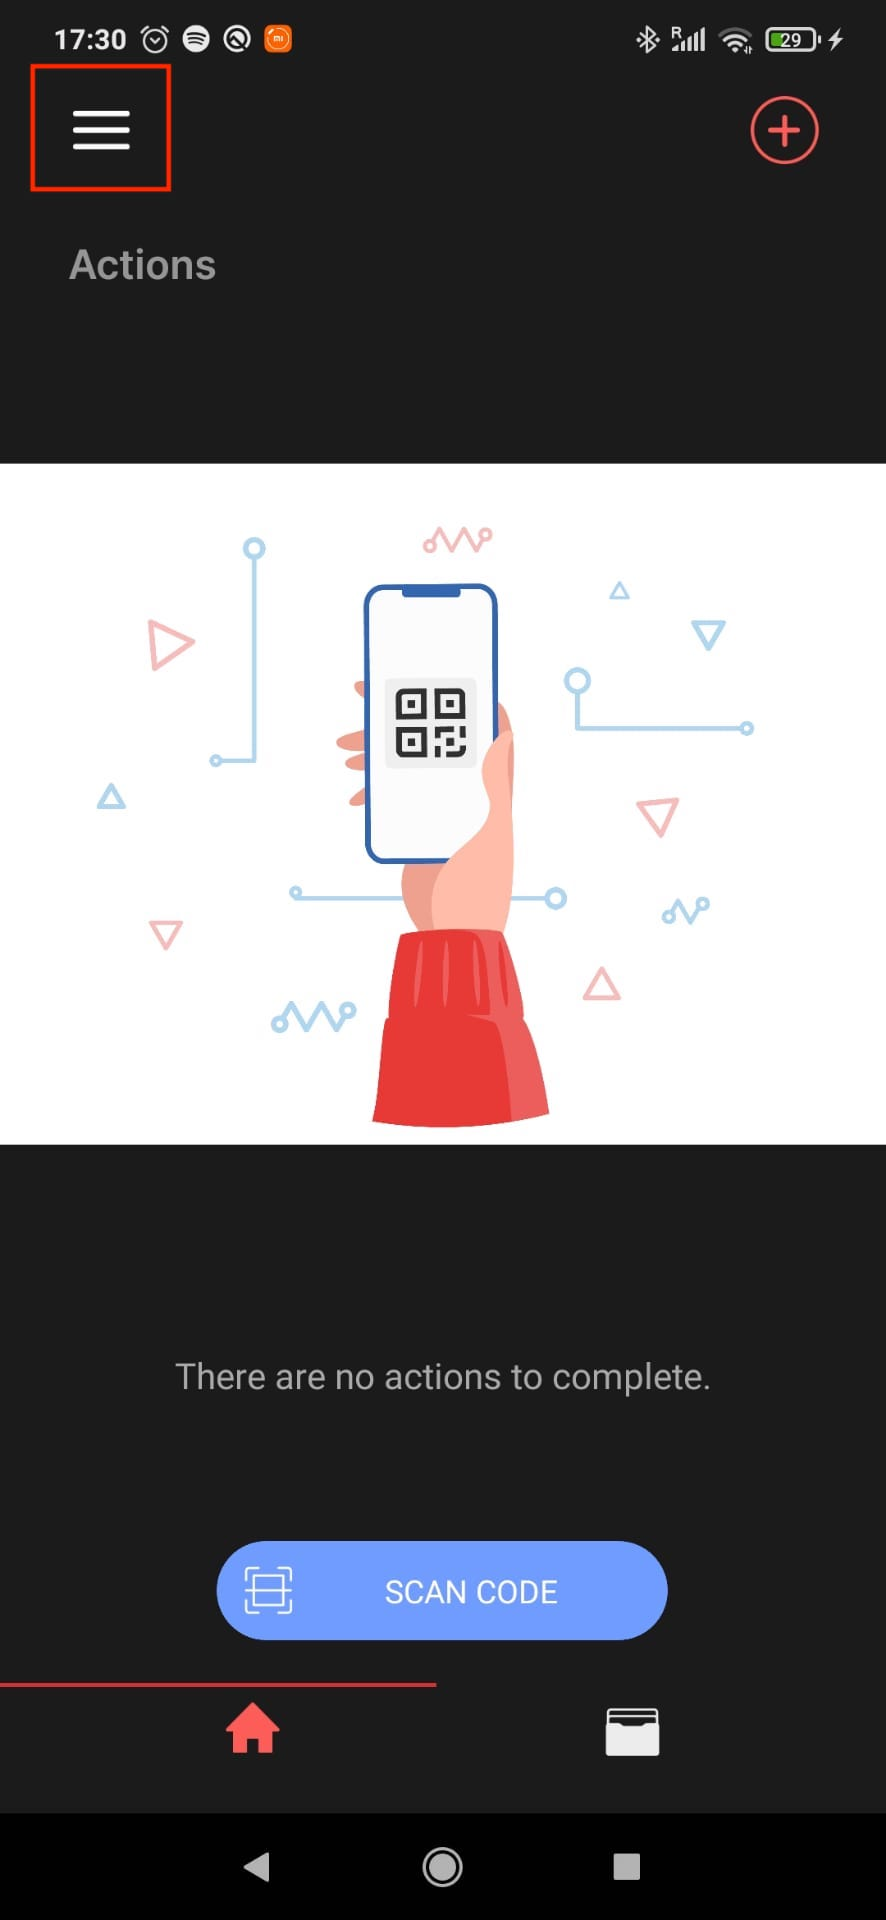
\includegraphics[width=\linewidth]{images/Trinsic/Trinsic_welcome_screen.jpeg}
  \caption[]{Go to Settings}\label{fig:trinsic_1}
\endminipage\hfill
\minipage{0.32\textwidth}
  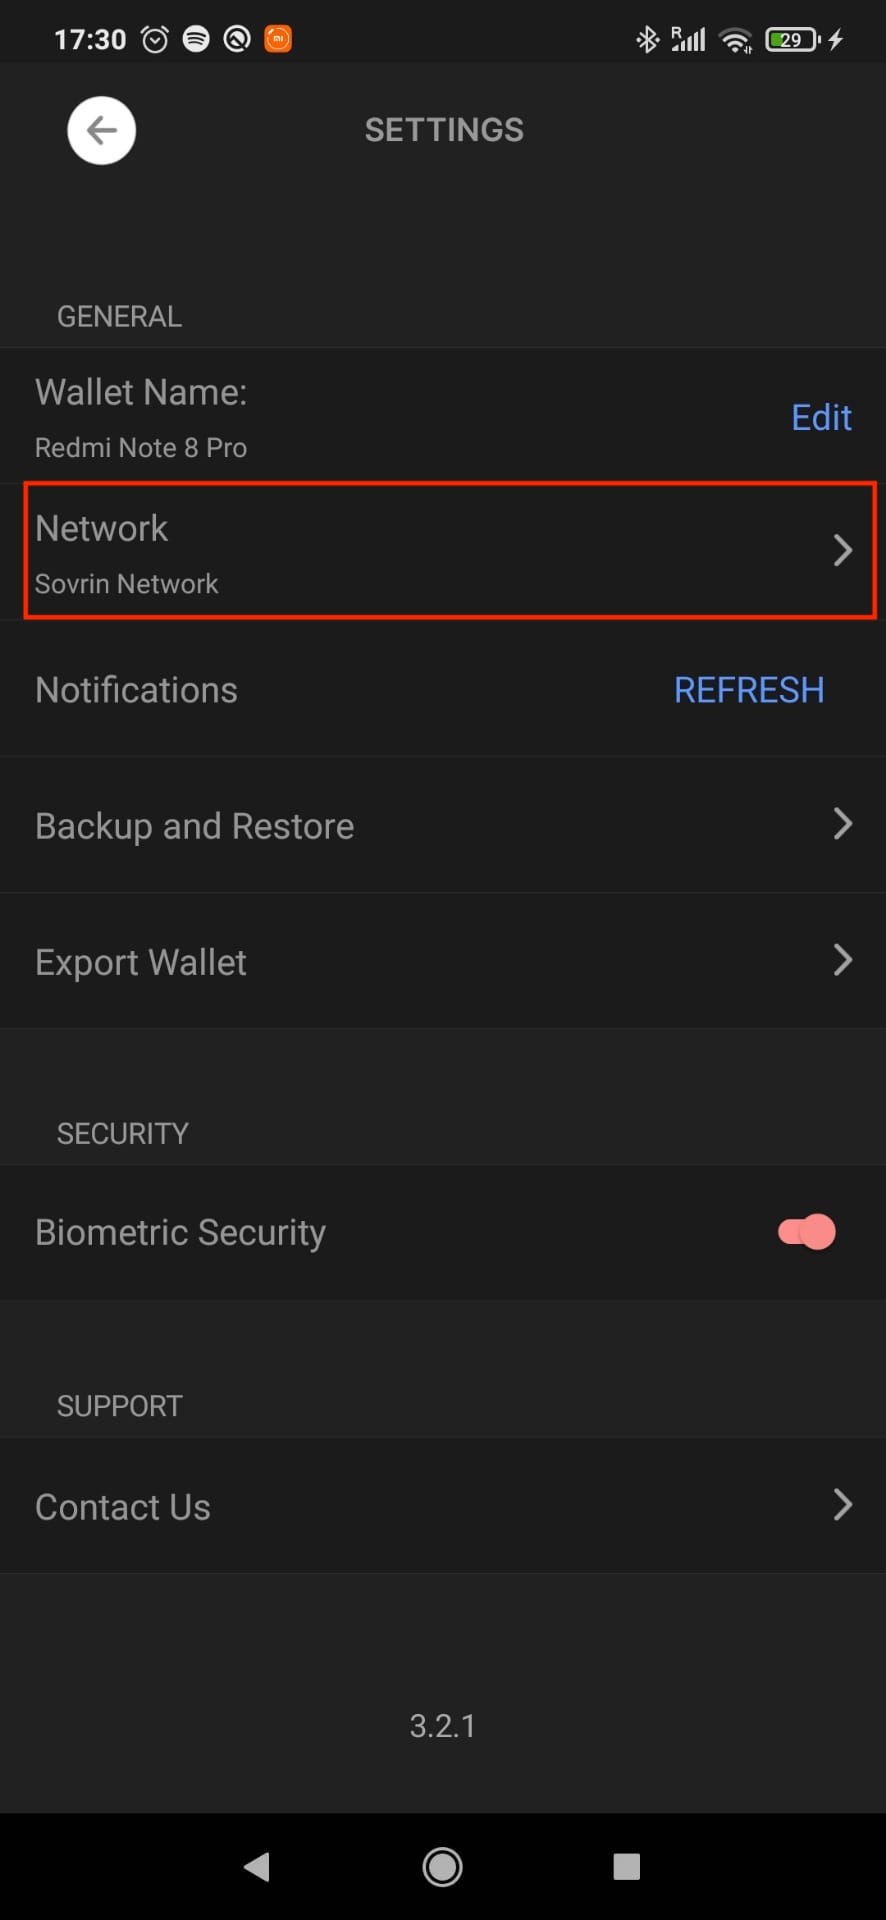
\includegraphics[width=\linewidth]{images/Trinsic/Trinsic_setup_network1.jpeg}
  \caption[]{Choose "Network" Option}\label{fig:trinsic_2}
\endminipage\hfill
\minipage{0.32\textwidth}%
  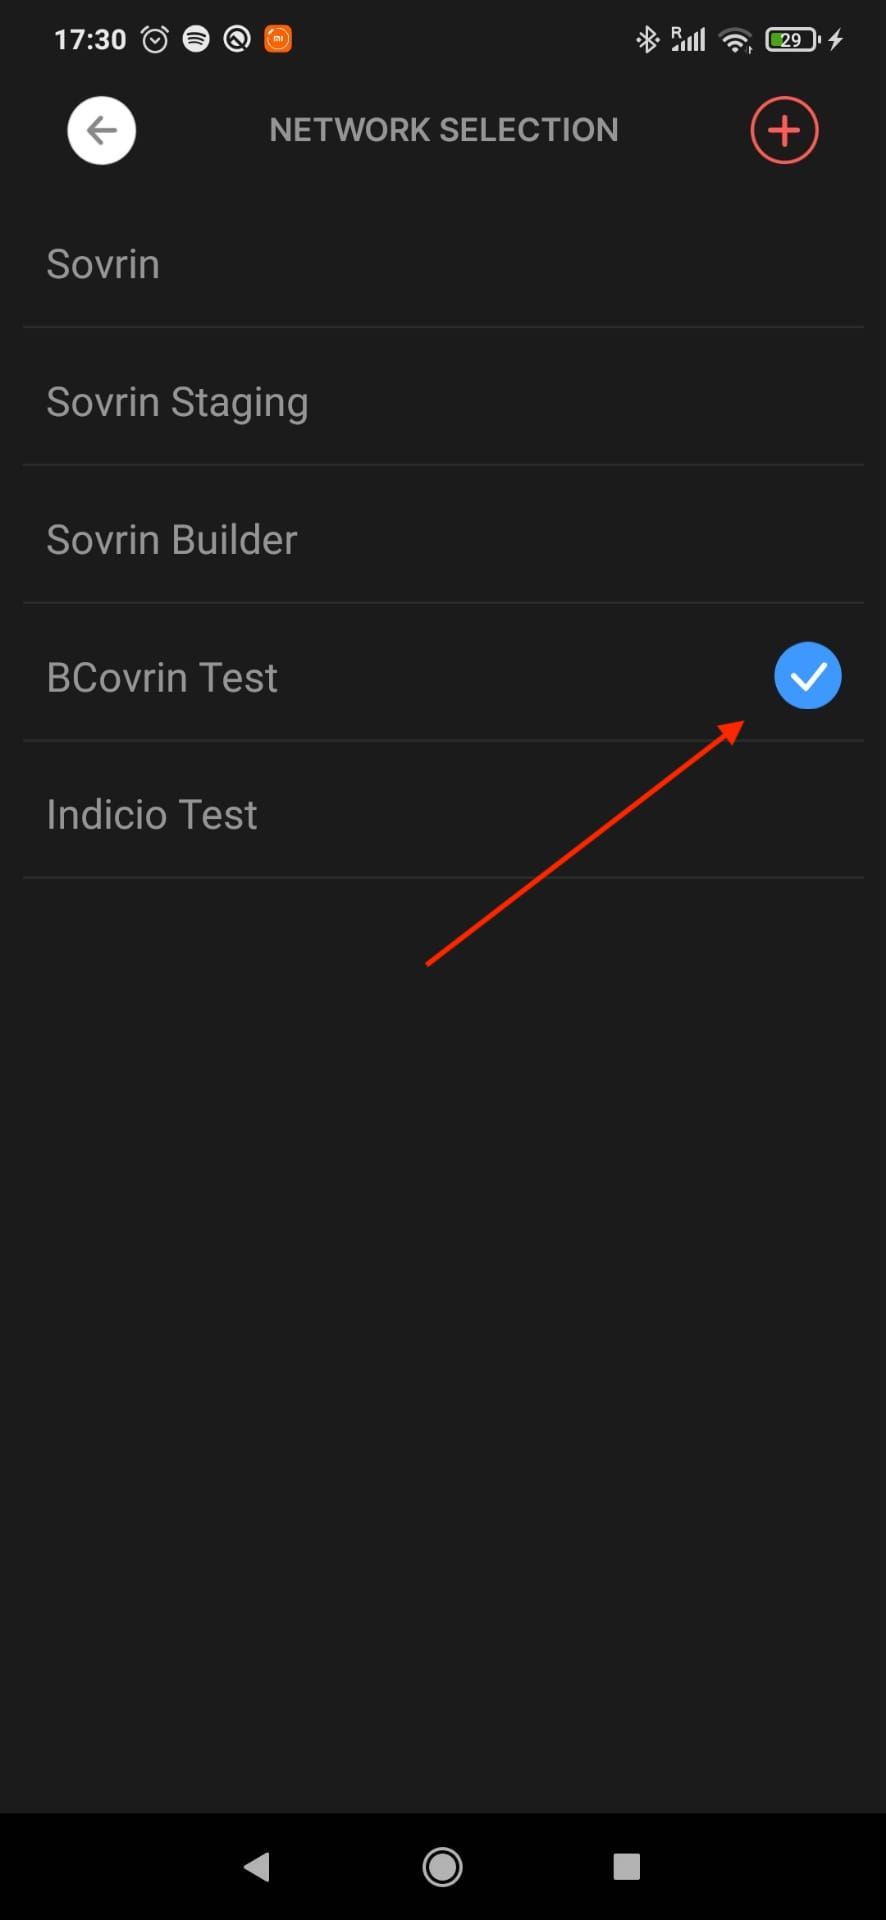
\includegraphics[width=\linewidth]{images/Trinsic/Trinsic_setup_network2.jpeg}
  \caption[]{Change it to "BCovrin Test"}\label{fig:trinsic_3}
\endminipage
\end{figure}

\newpage    % I wanted each new appendix to start on a new page

\subsection{Application Screenshots}
\label{app:application_screenshots}

In this appendix the screenshots of the frontend as well as from the Trinsic Wallet App on the EV Owner's phone are presented, to illustrate each step of each use-case.

\subsubsection{Service Providers Flow with SSI Screenshots}
\label{subapp:service_providers_flow}

\begin{figure}[H]
    \centering
    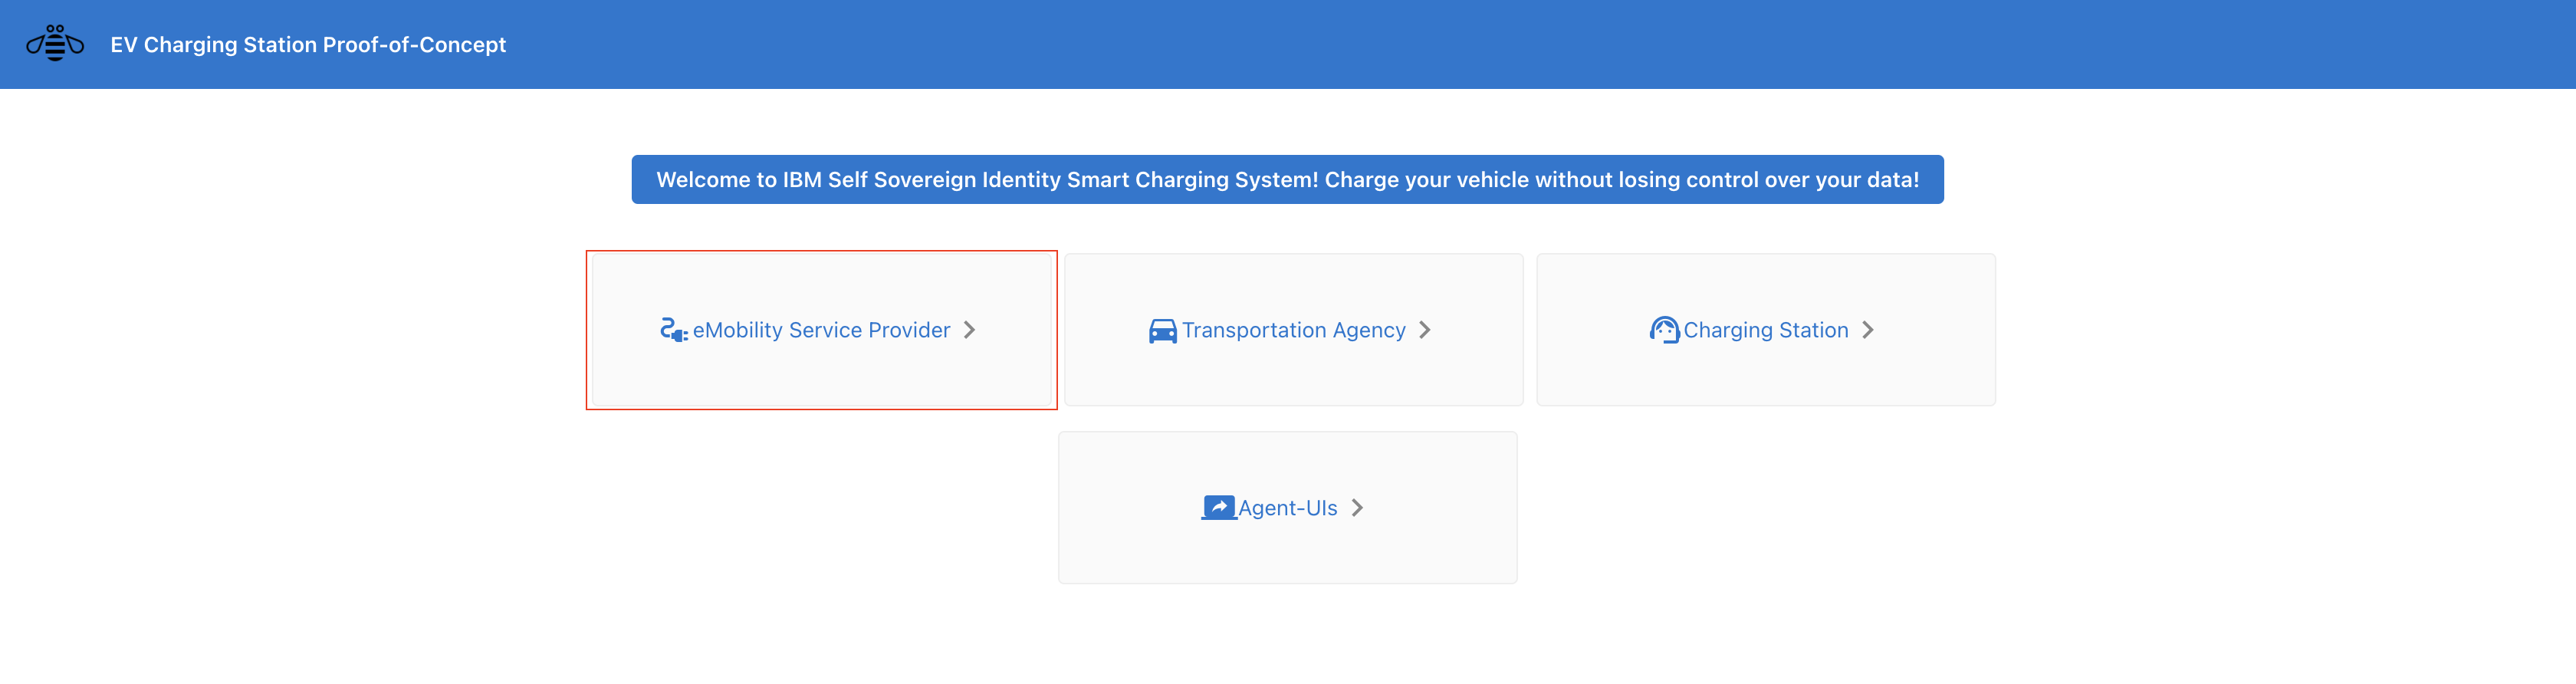
\includegraphics[width=\linewidth]{images/Frontend/eMSP/Screenshot1.png}
    \caption[]{Selecting eMSP portal}
    \label{fig:service_provider_screenshot_1}
\end{figure}

\begin{figure}[H]
\centering
\begin{minipage}{.5\textwidth}
  \centering
  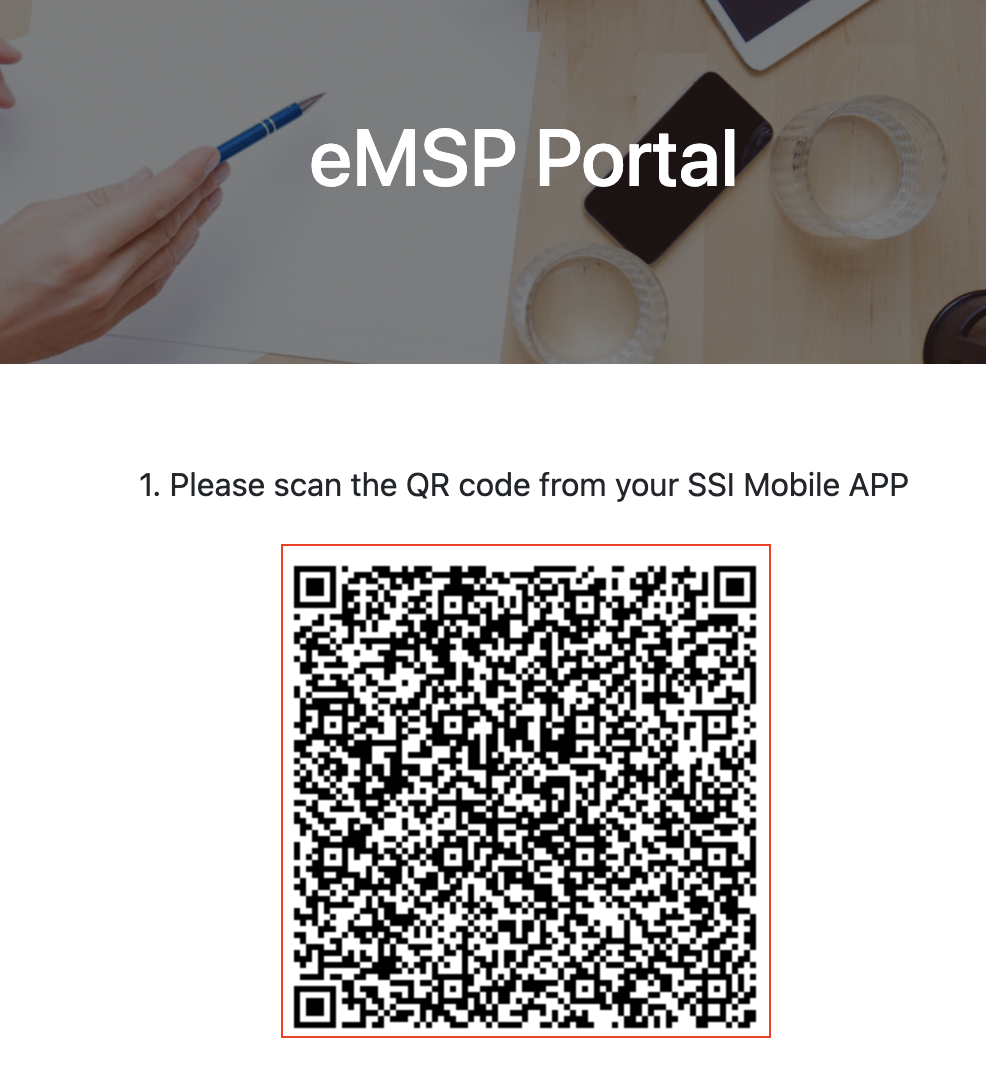
\includegraphics[width=.8\linewidth]{images/Frontend/eMSP/Screenshot2.png}
  \caption[]{Connect to eMSP Agent using QR Code}
  \label{fig:service_provider_screenshot_2}
\end{minipage}%
\begin{minipage}{.5\textwidth}
  \centering
  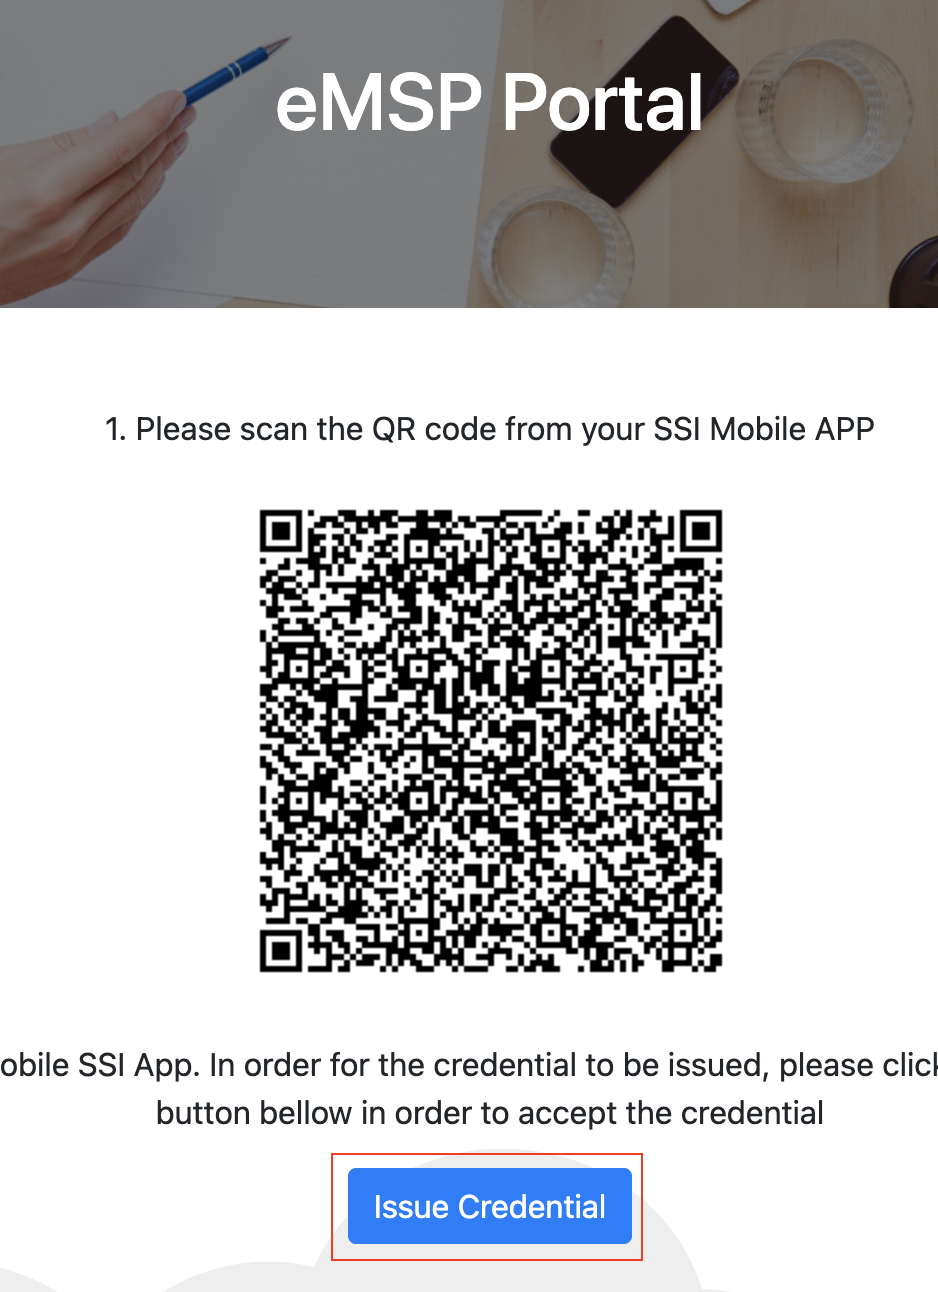
\includegraphics[width=.8\linewidth]{images/Frontend/eMSP/Screenshot3.png}
  \caption[]{Press the "Issue Credential" button}
  \label{fig:service_provider_screenshot_3}
\end{minipage}
\end{figure}

\begin{figure}[H]
    \centering
    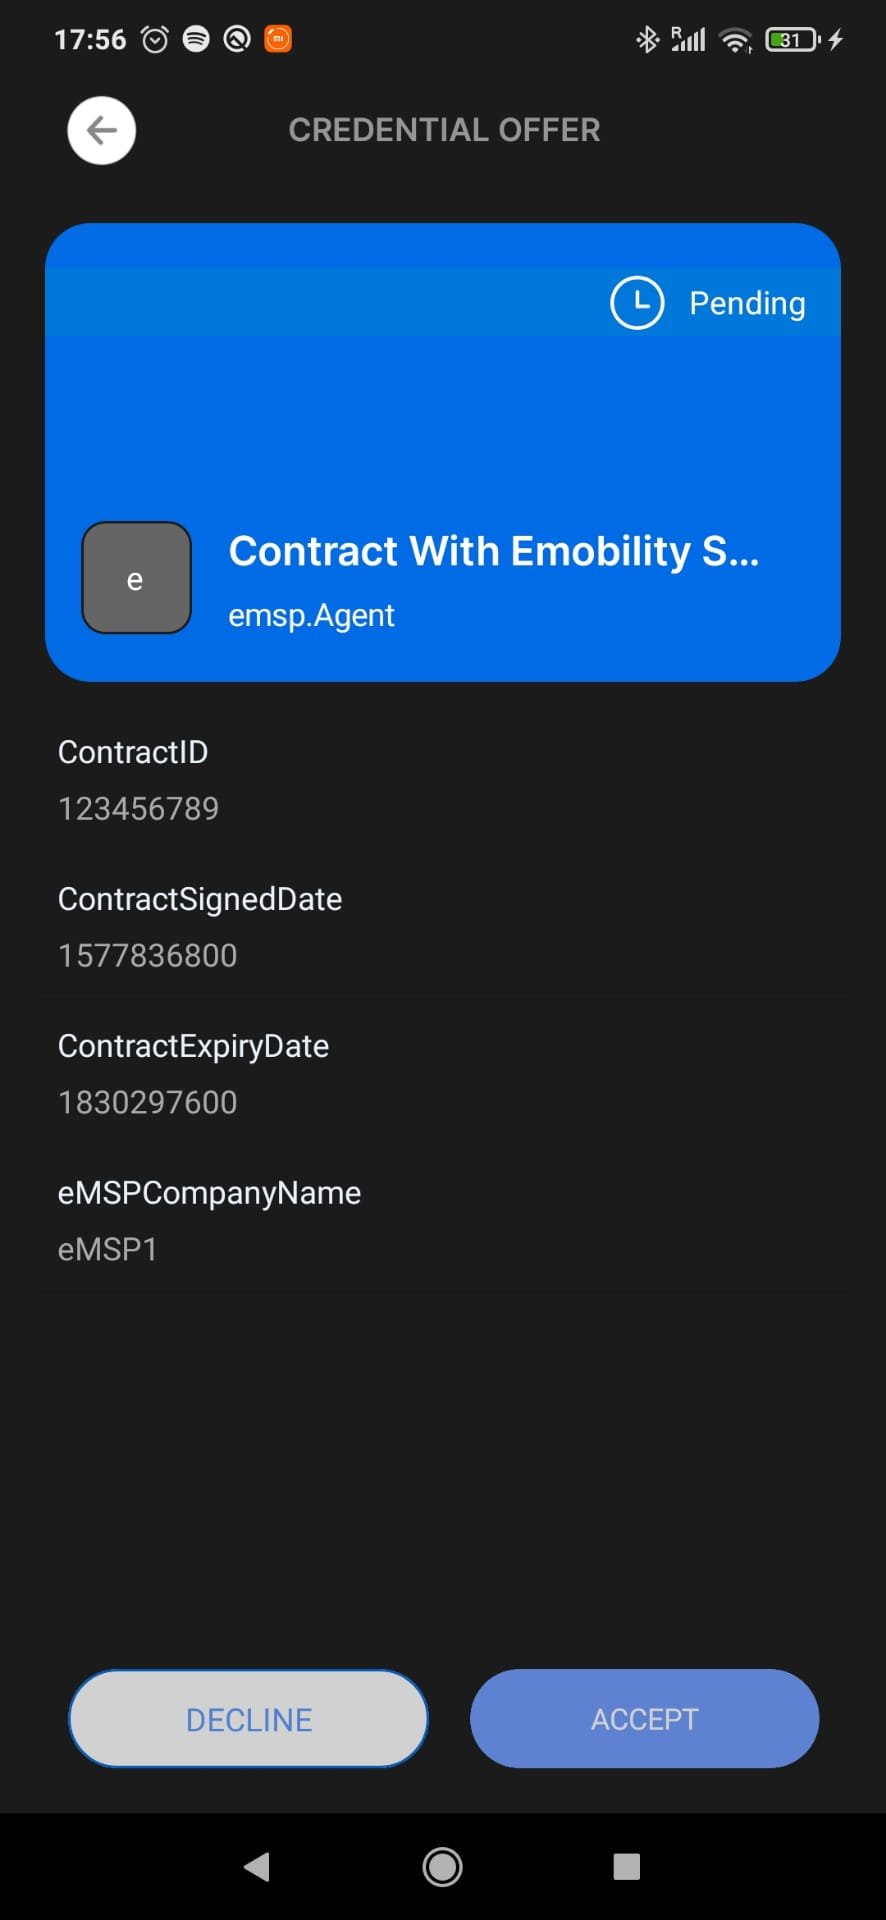
\includegraphics[width=0.4\linewidth]{images/Frontend/eMSP/Screenshot4.jpeg}
    \caption[]{Accept the credential on the Trinsic Wallet App}
    \label{fig:service_provider_screenshot_4}
\end{figure}

\newpage

\subsubsection{EV Owner and EV Interactions with SSI Screenshots}
\label{subapp:ev_owner_and_ev_interactions}

\begin{figure}[H]
    \centering
    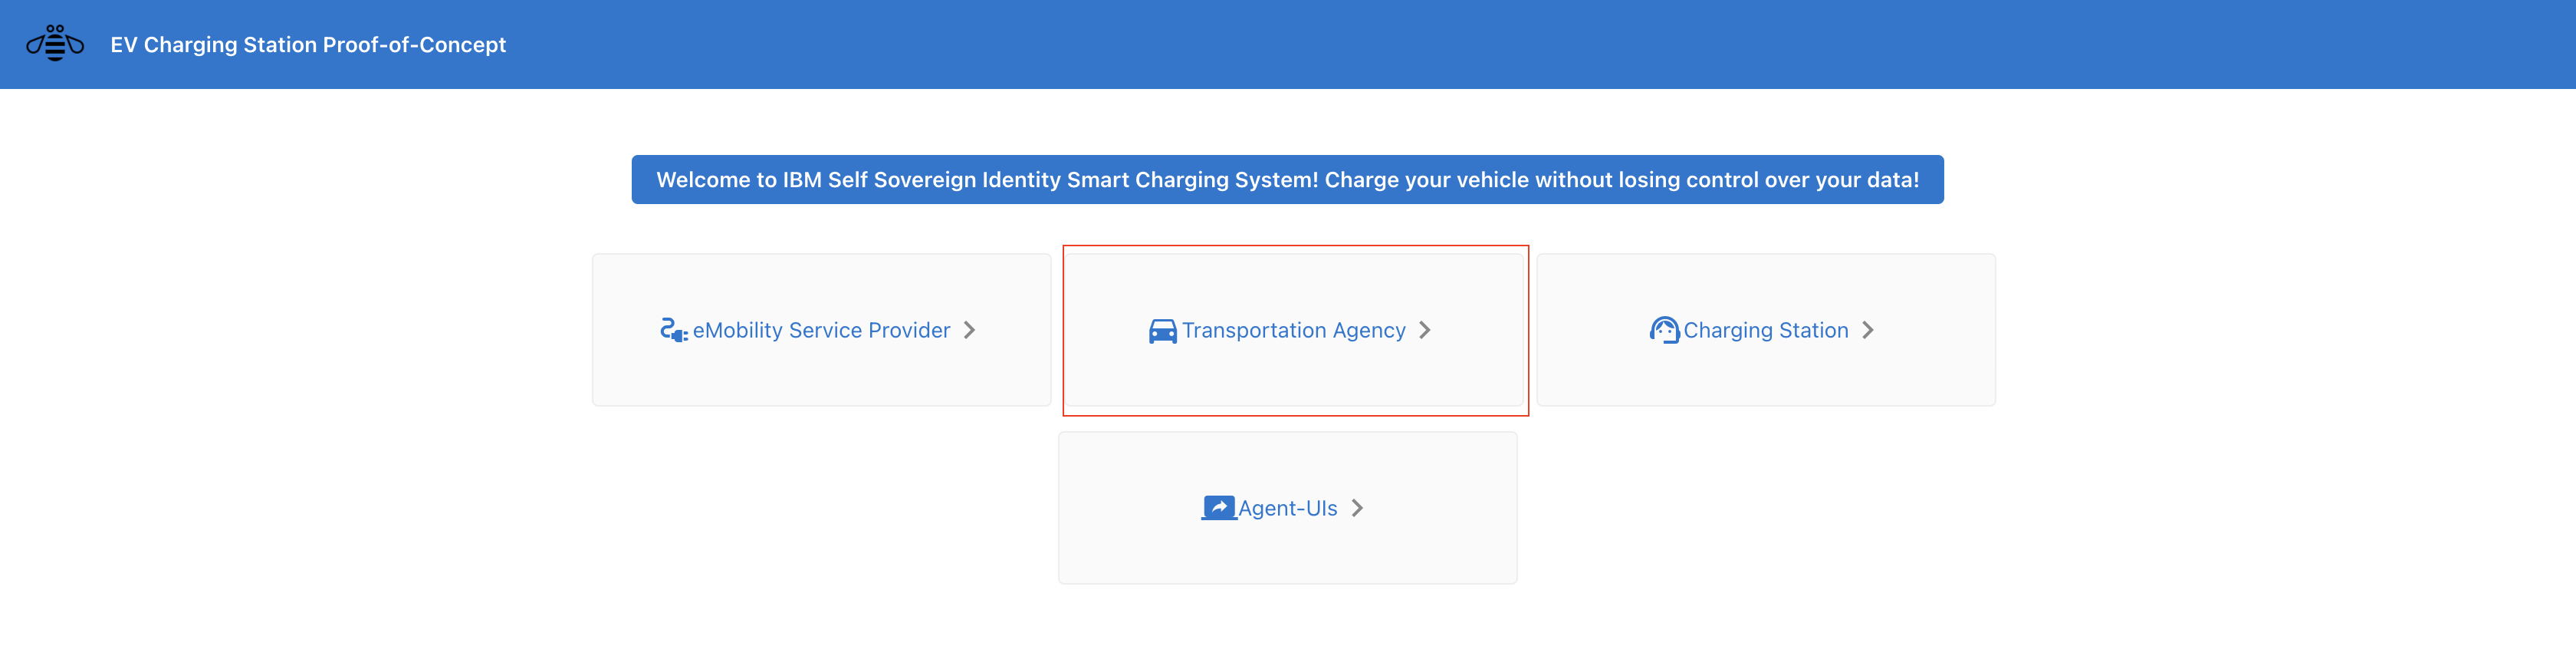
\includegraphics[width=\linewidth]{images/Frontend/Transportation_agency/Screenshot1.png}
    \caption[]{Selecting Transportation Agency portal}
    \label{fig:ev_owner_screenshot_1}
\end{figure}

\begin{figure}[H]
\centering
\begin{minipage}{.5\textwidth}
  \centering
  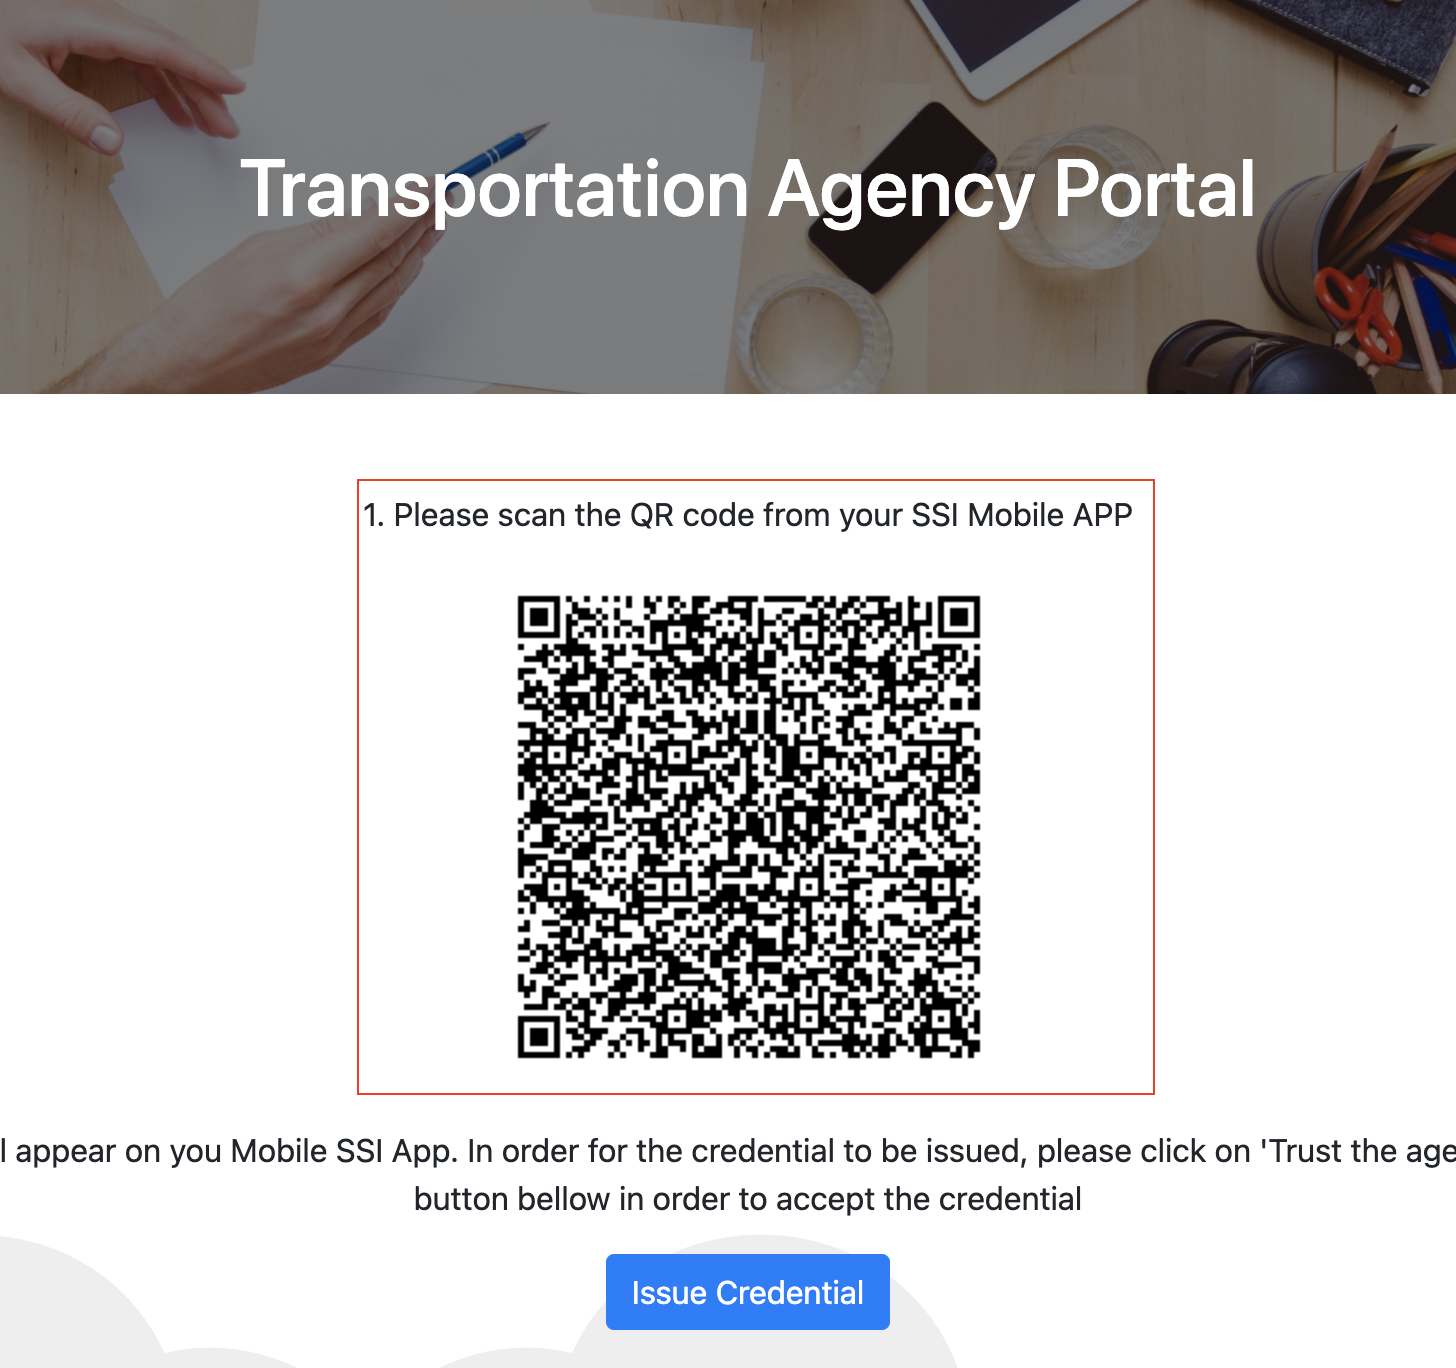
\includegraphics[width=.8\linewidth]{images/Frontend/Transportation_agency/Screenshot2.png}
  \caption[]{Connect to Transportation Agency Agent using QR Code}
  \label{fig:ev_owner_screenshot_2}
\end{minipage}%
\begin{minipage}{.5\textwidth}
  \centering
  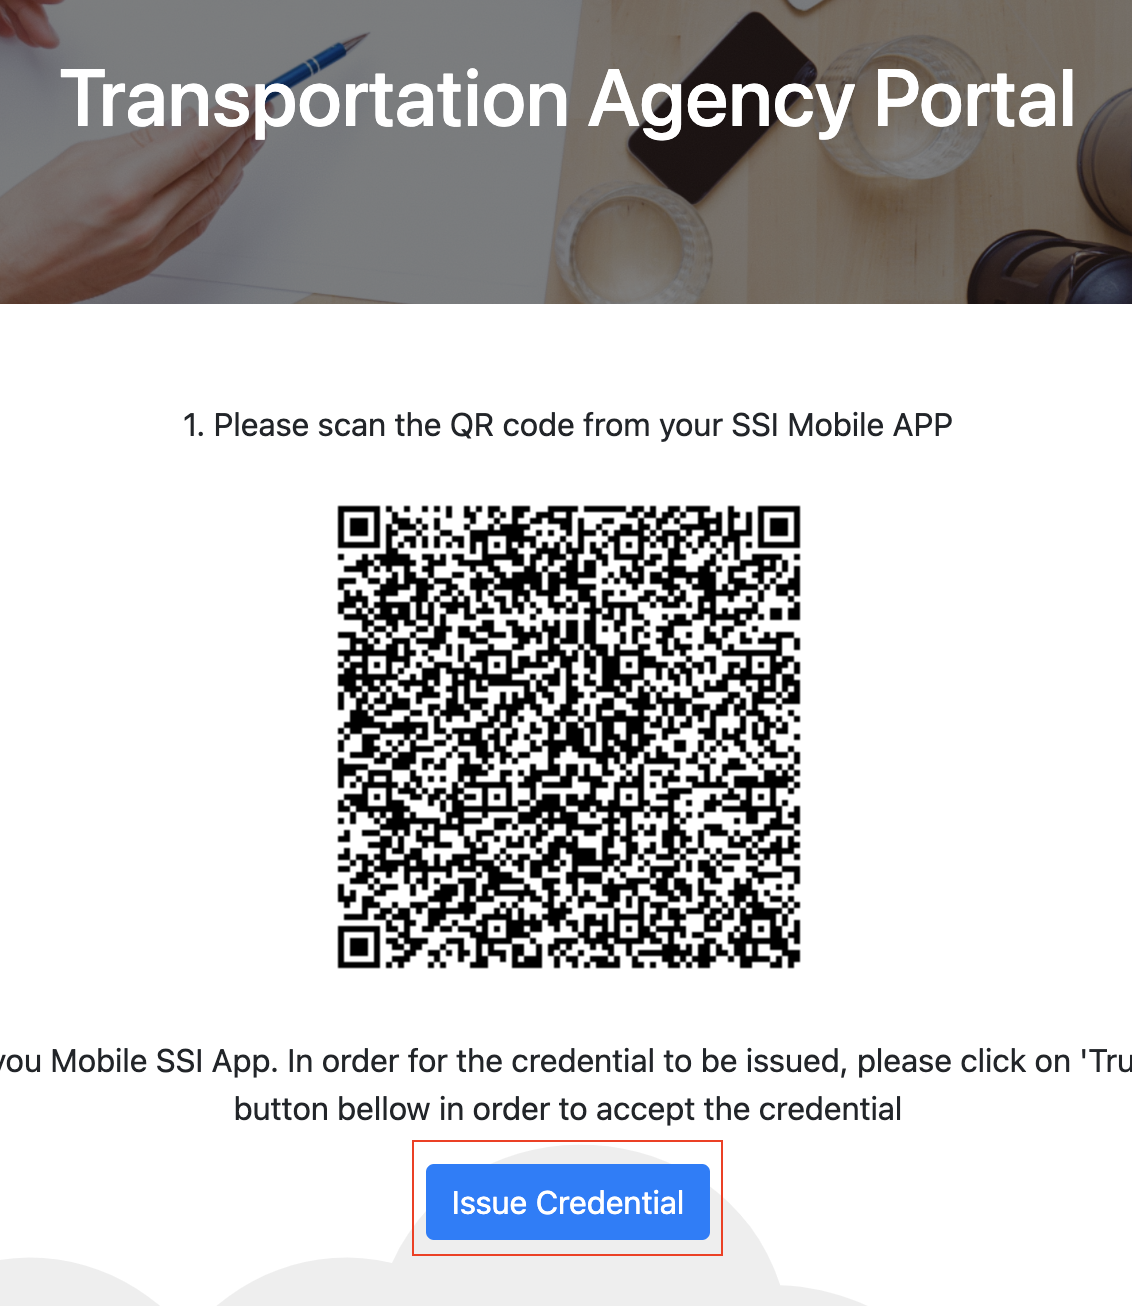
\includegraphics[width=.8\linewidth]{images/Frontend/Transportation_agency/Screenshot3.png}
  \caption[]{Press the "Issue Credential" button}
  \label{fig:ev_owner_screenshot_3}
\end{minipage}
\end{figure}

\begin{figure}[H]
    \centering
    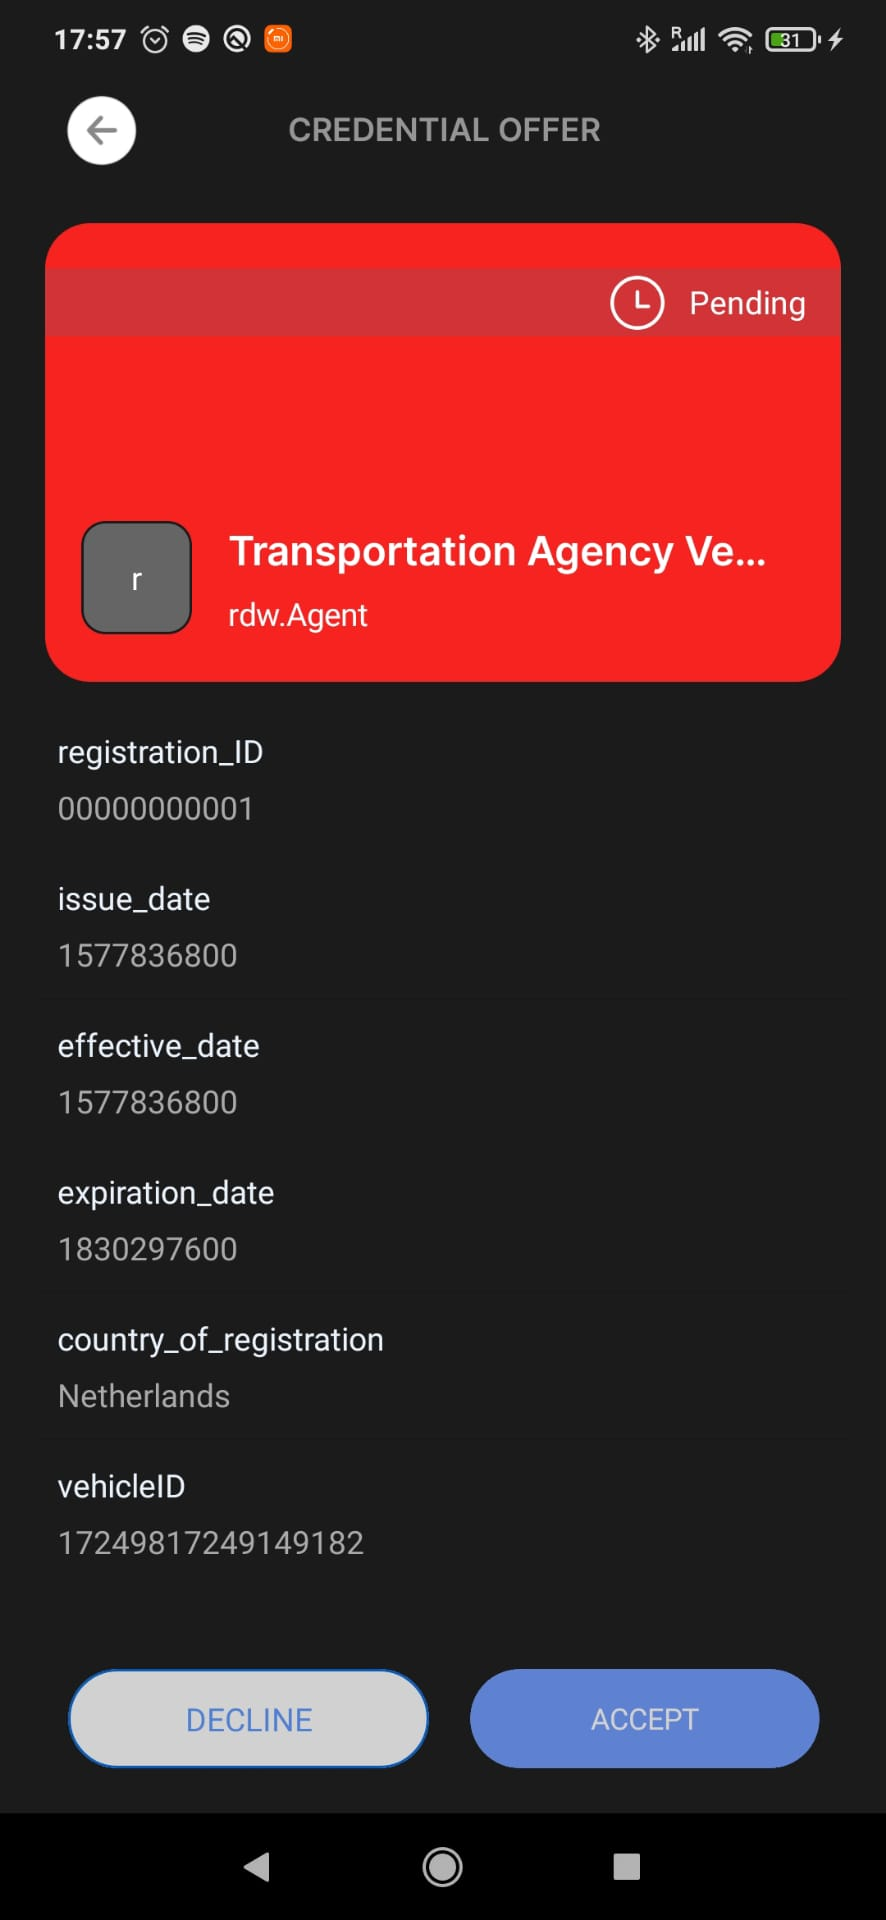
\includegraphics[width=0.4\linewidth]{images/Frontend/Transportation_agency/Screenshot4.jpeg}
    \caption[]{Accept the credential on the Trinsic Wallet App}
    \label{fig:ev_owner_screenshot_4}
\end{figure}

\newpage

\subsubsection{Charging and Billing with SSI Screenshots}
\label{subapp:charging_and_billing}

\begin{figure}[H]
    \centering
    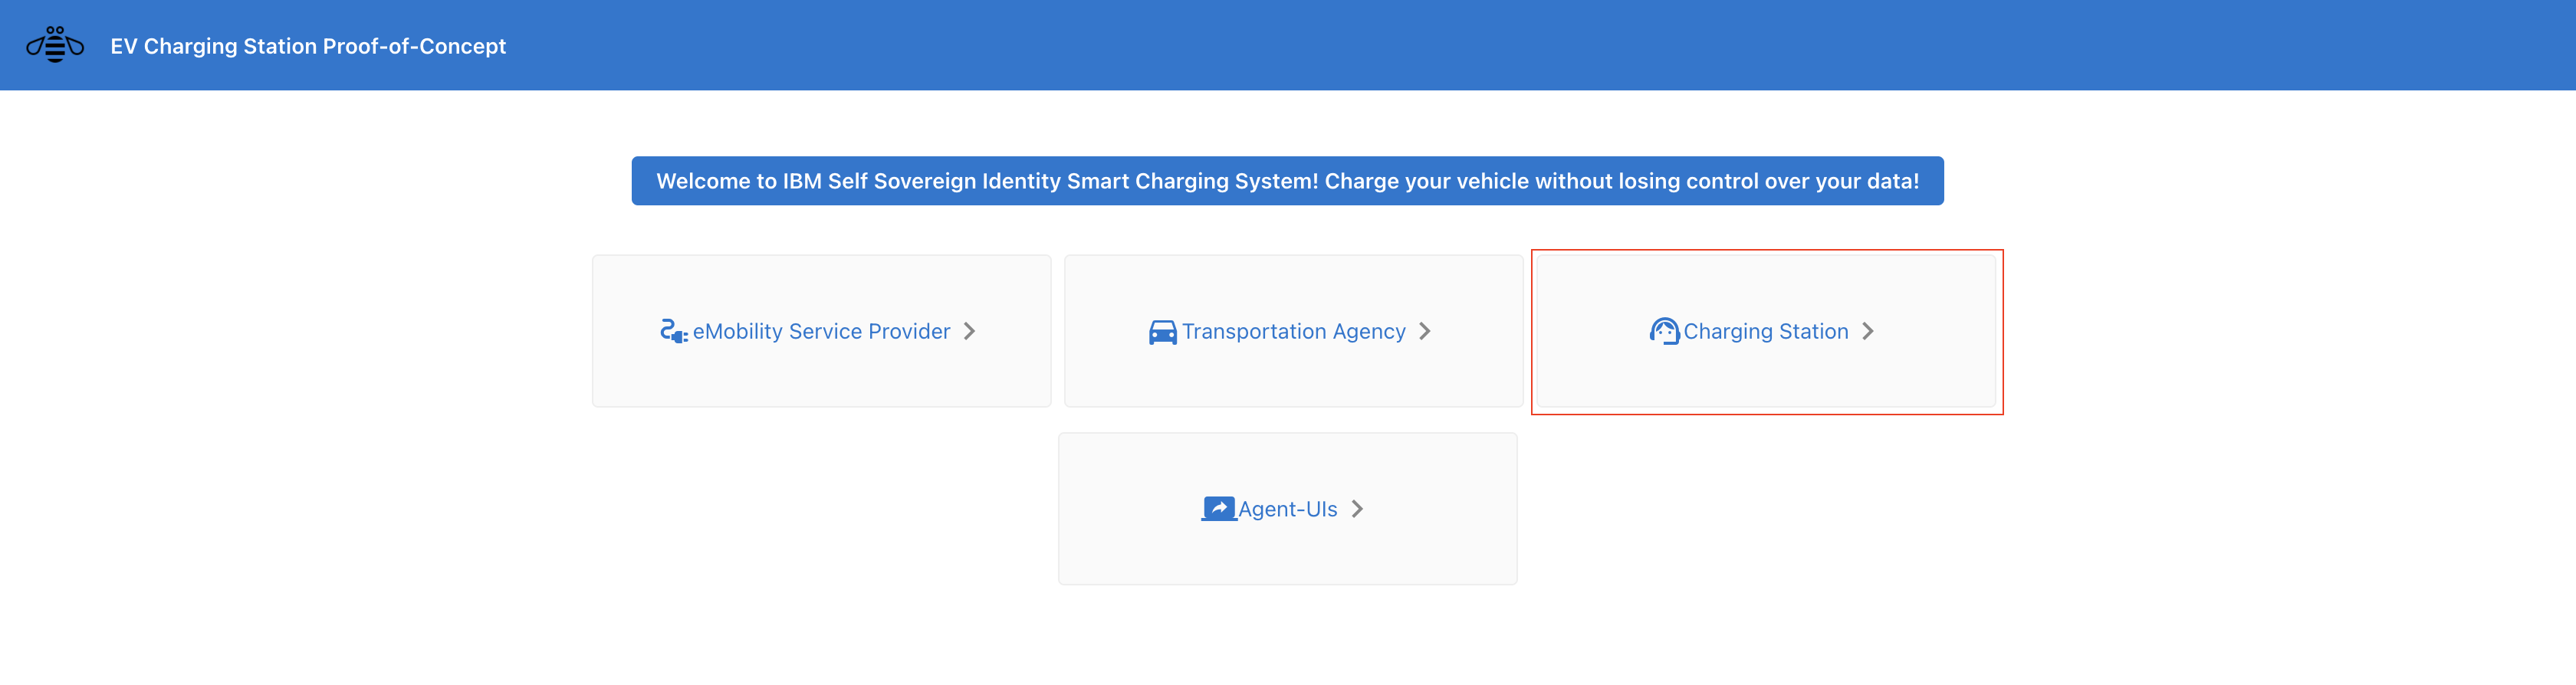
\includegraphics[width=\linewidth]{images/Frontend/Charging/1.0.png}
    \caption[]{Selecting Charging Station dashboard}
    \label{fig:charging_screenshot_1.0}
\end{figure}

\begin{figure}[H]
\centering
\begin{minipage}{.5\textwidth}
  \centering
  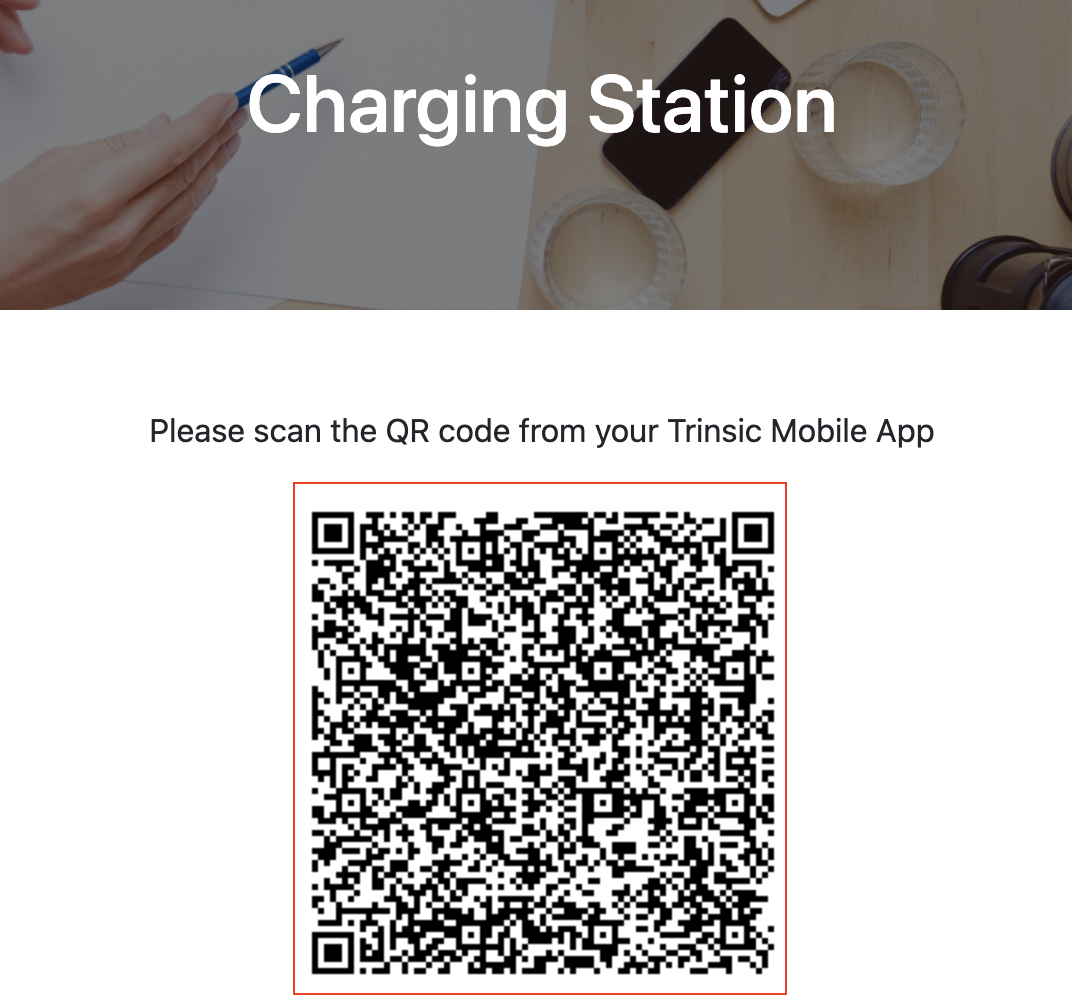
\includegraphics[width=.9\linewidth]{images/Frontend/Charging/1.1.png}
  \caption[]{Connect  to Charging Station Agent  using  QRCode}
  \label{fig:charging_screenshot_1.1}
\end{minipage}%
\begin{minipage}{.5\textwidth}
  \centering
  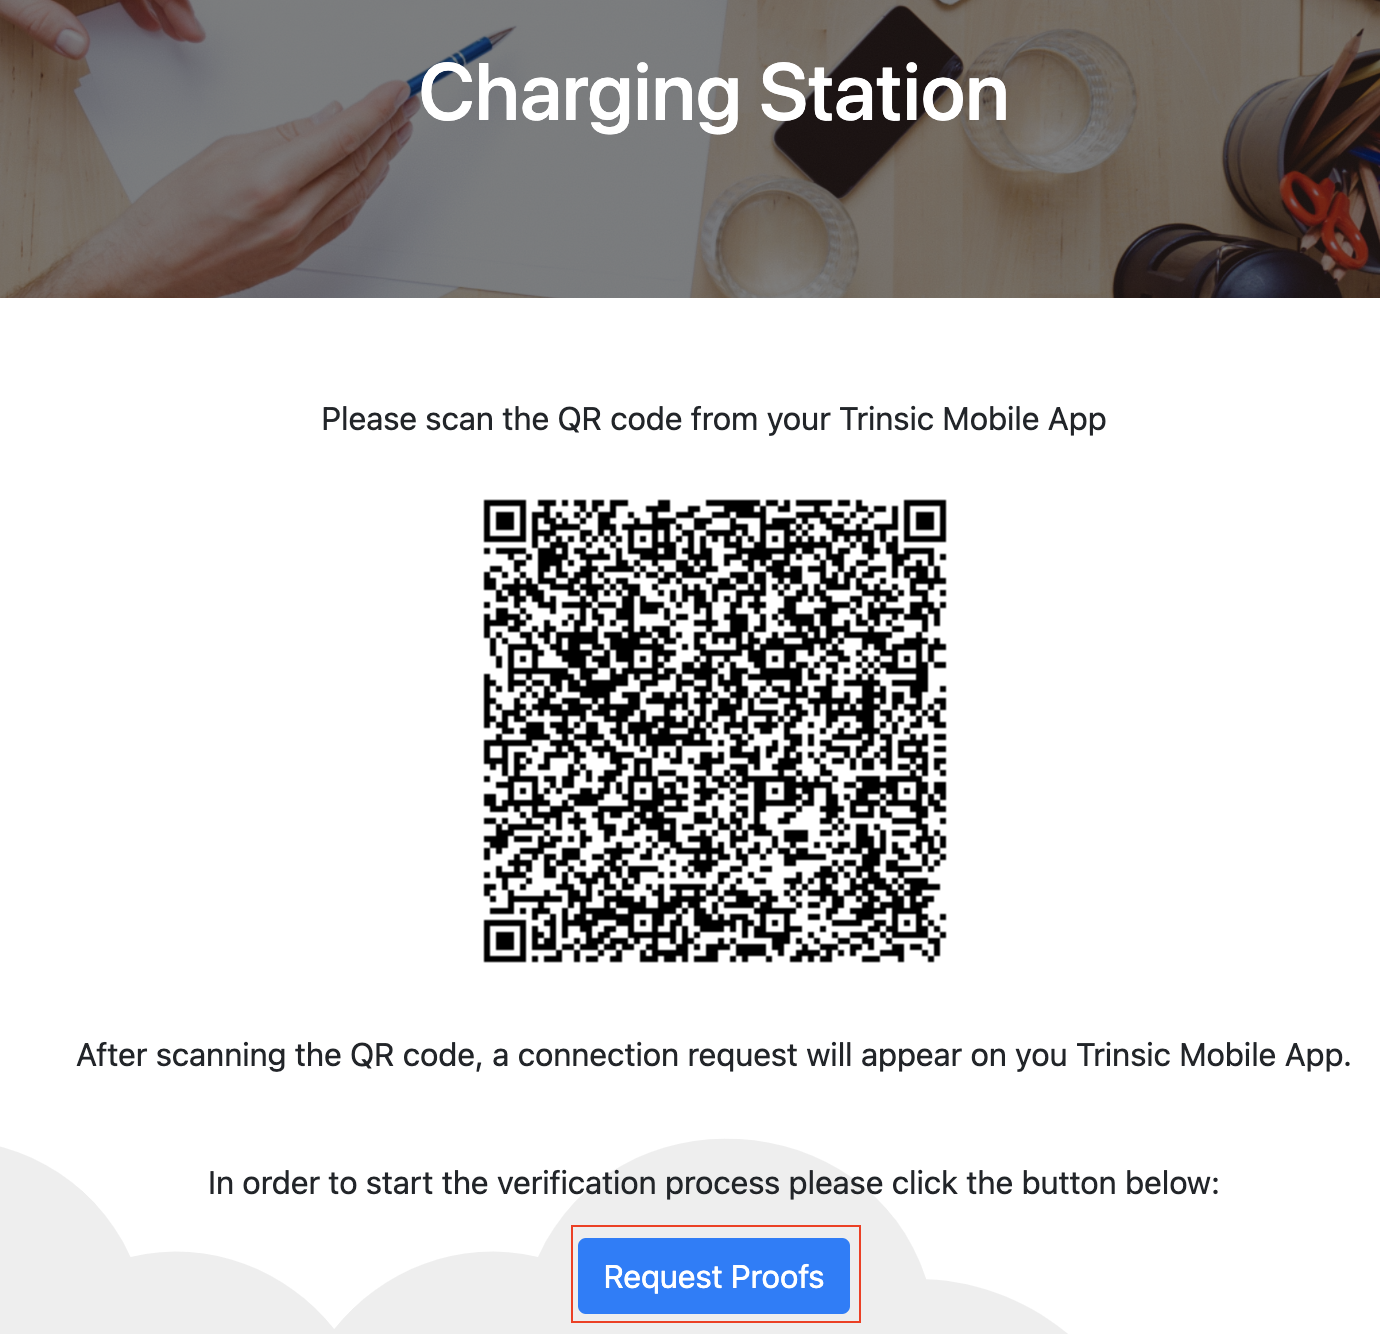
\includegraphics[width=.9\linewidth]{images/Frontend/Charging/2.png}
  \caption[]{Press the "Request Proofs" button}
  \label{fig:charging_screenshot_2}
\end{minipage}
\end{figure}

\begin{figure}[H]
\centering
\begin{minipage}{.33\textwidth}
  \centering
  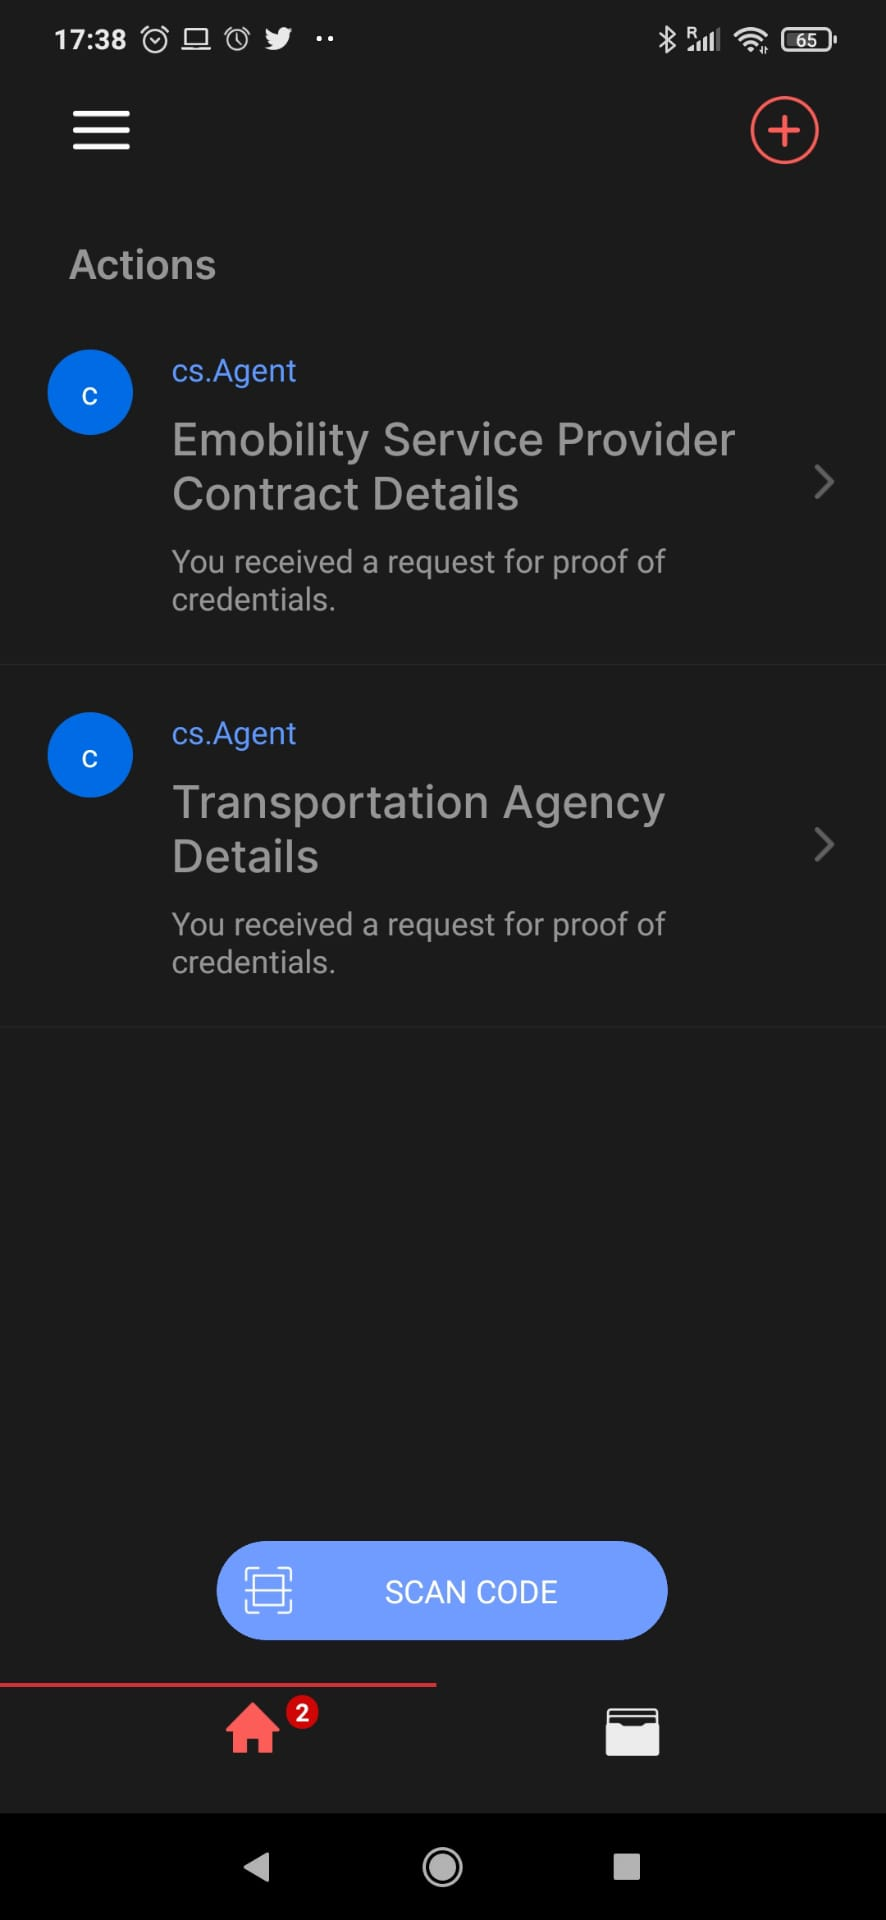
\includegraphics[width=.8\linewidth]{images/Frontend/Charging/3.0.jpeg}
  \caption[]{Receive Presentation Proof Requests on Trinsic Wallet App}
  \label{fig:charging_screenshot_3}
\end{minipage}%
\begin{minipage}{.33\textwidth}
  \centering
  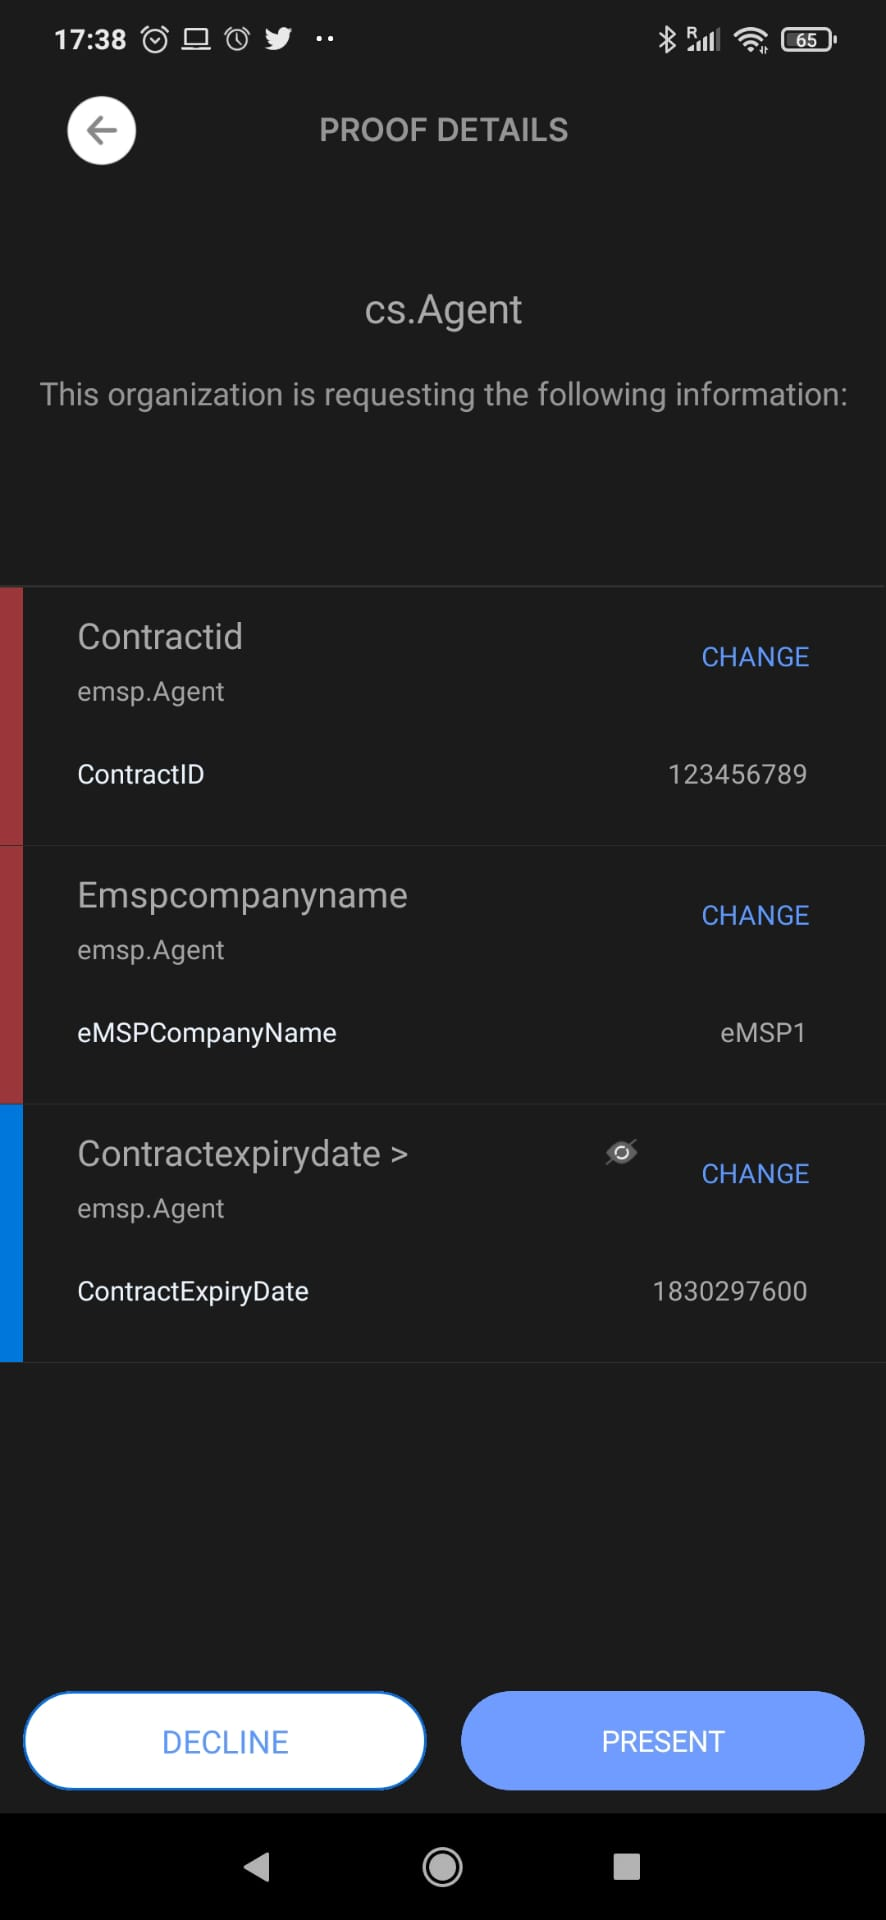
\includegraphics[width=.8\linewidth]{images/Frontend/Charging/3.1.jpeg}
  \caption[]{Present the proof for the TA-issued credential}
  \label{fig:charging_screenshot_3.1}
\end{minipage}
\begin{minipage}{.33\textwidth}
  \centering
  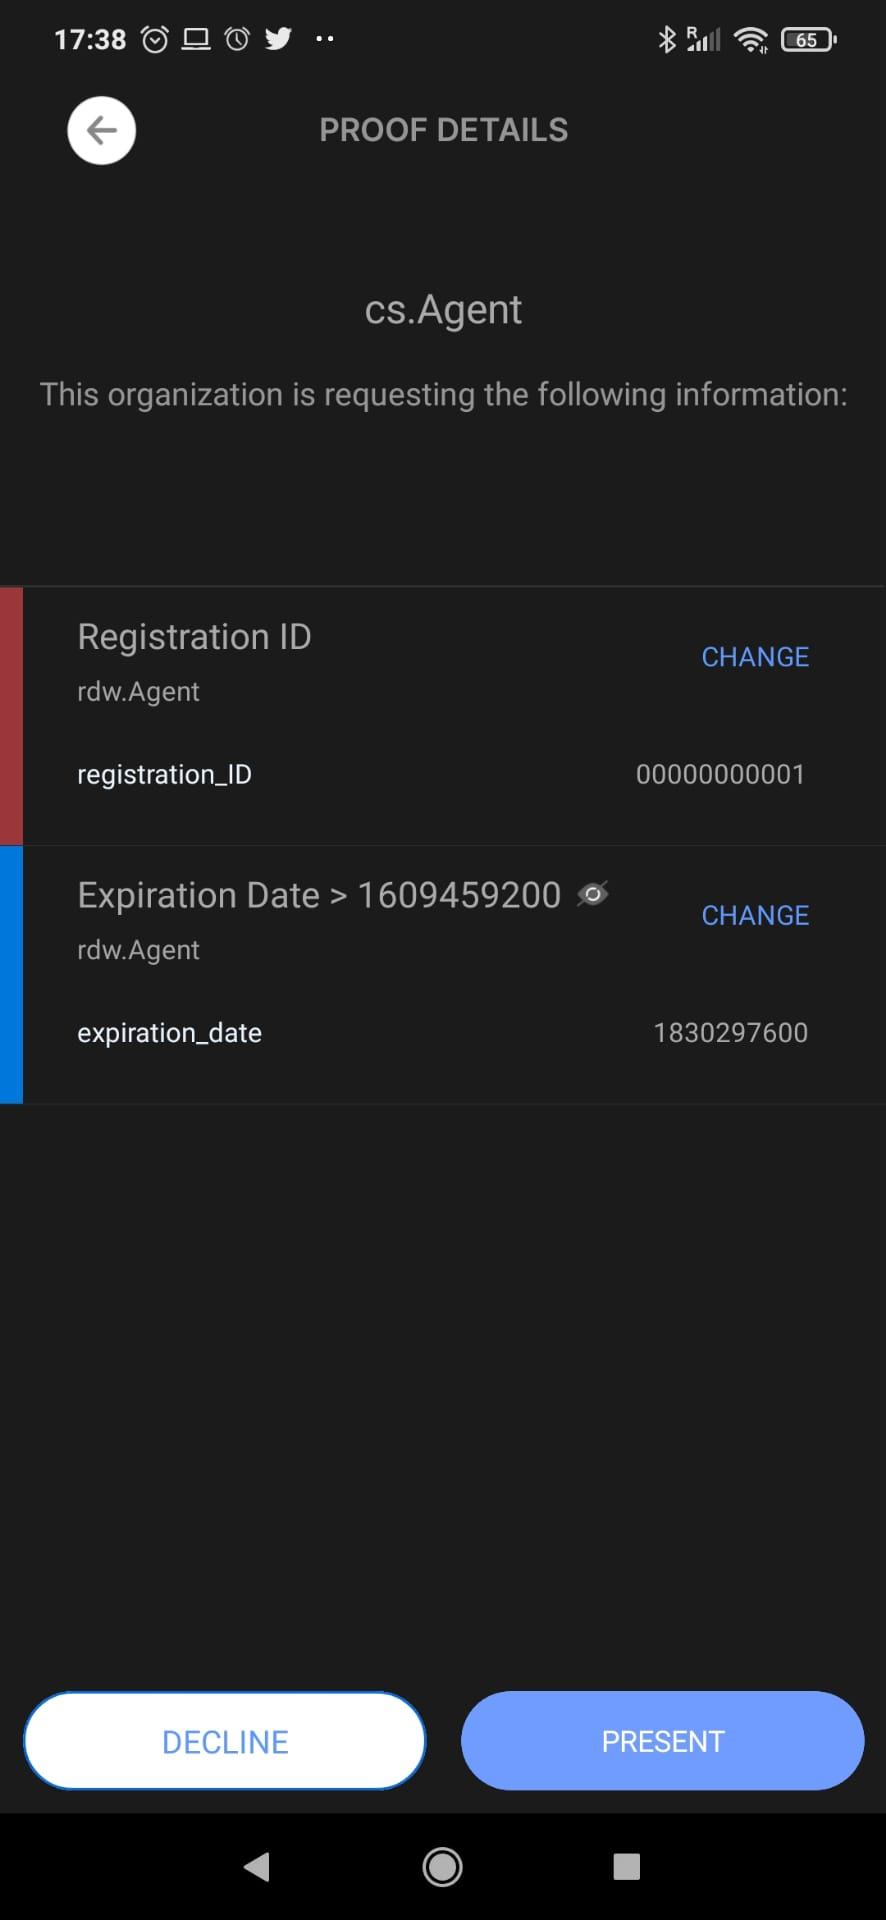
\includegraphics[width=.8\linewidth]{images/Frontend/Charging/3.2.jpeg}
  \caption[]{Present the proof for the eMSP-issued credential}
  \label{fig:charging_screenshot_3.2}
\end{minipage}
\end{figure}

\begin{figure}[H]
\centering
\begin{minipage}{.5\textwidth}
  \centering
  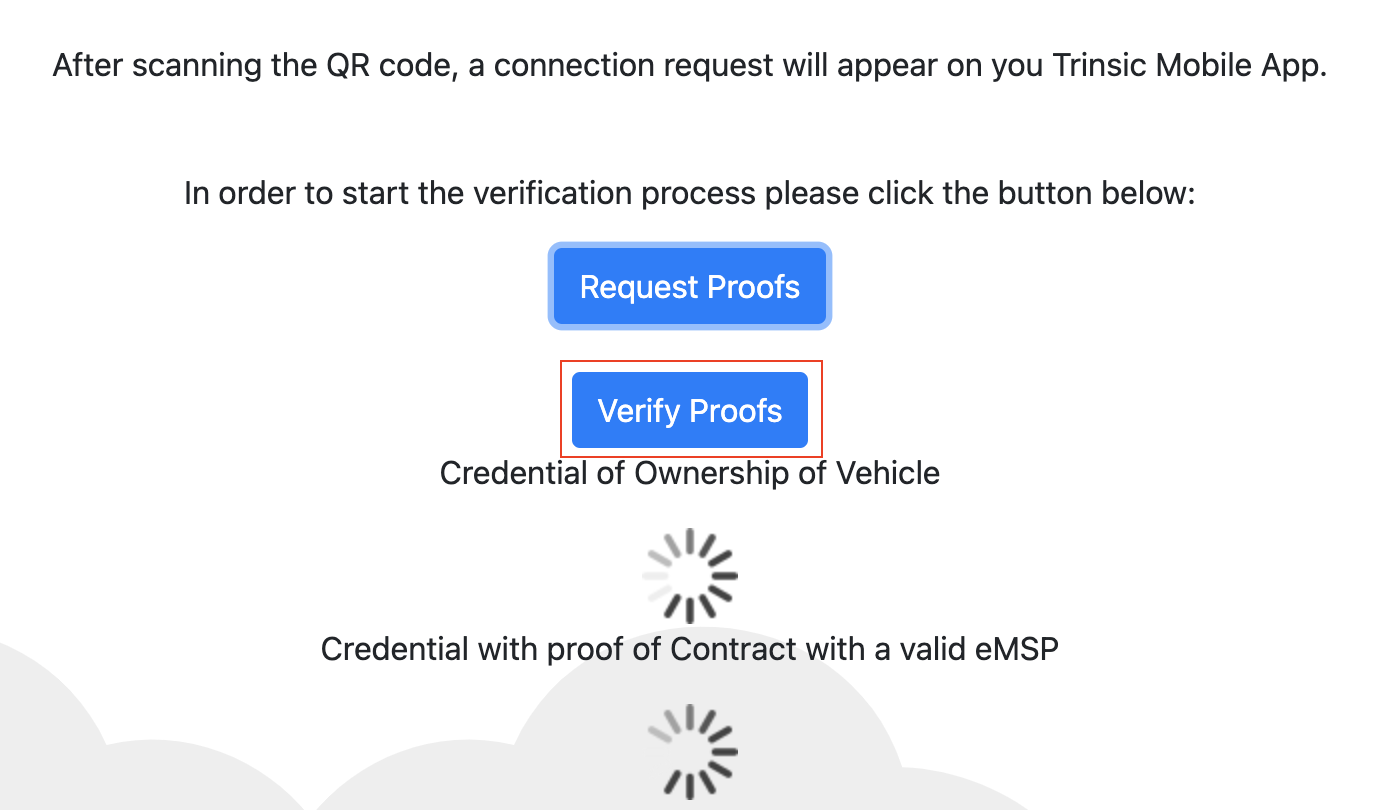
\includegraphics[width=.9\linewidth]{images/Frontend/Charging/4.png}
  \caption[]{Press the "Verify Proofs" button}
  \label{fig:charging_screenshot_4}
\end{minipage}%
\begin{minipage}{.5\textwidth}
  \centering
  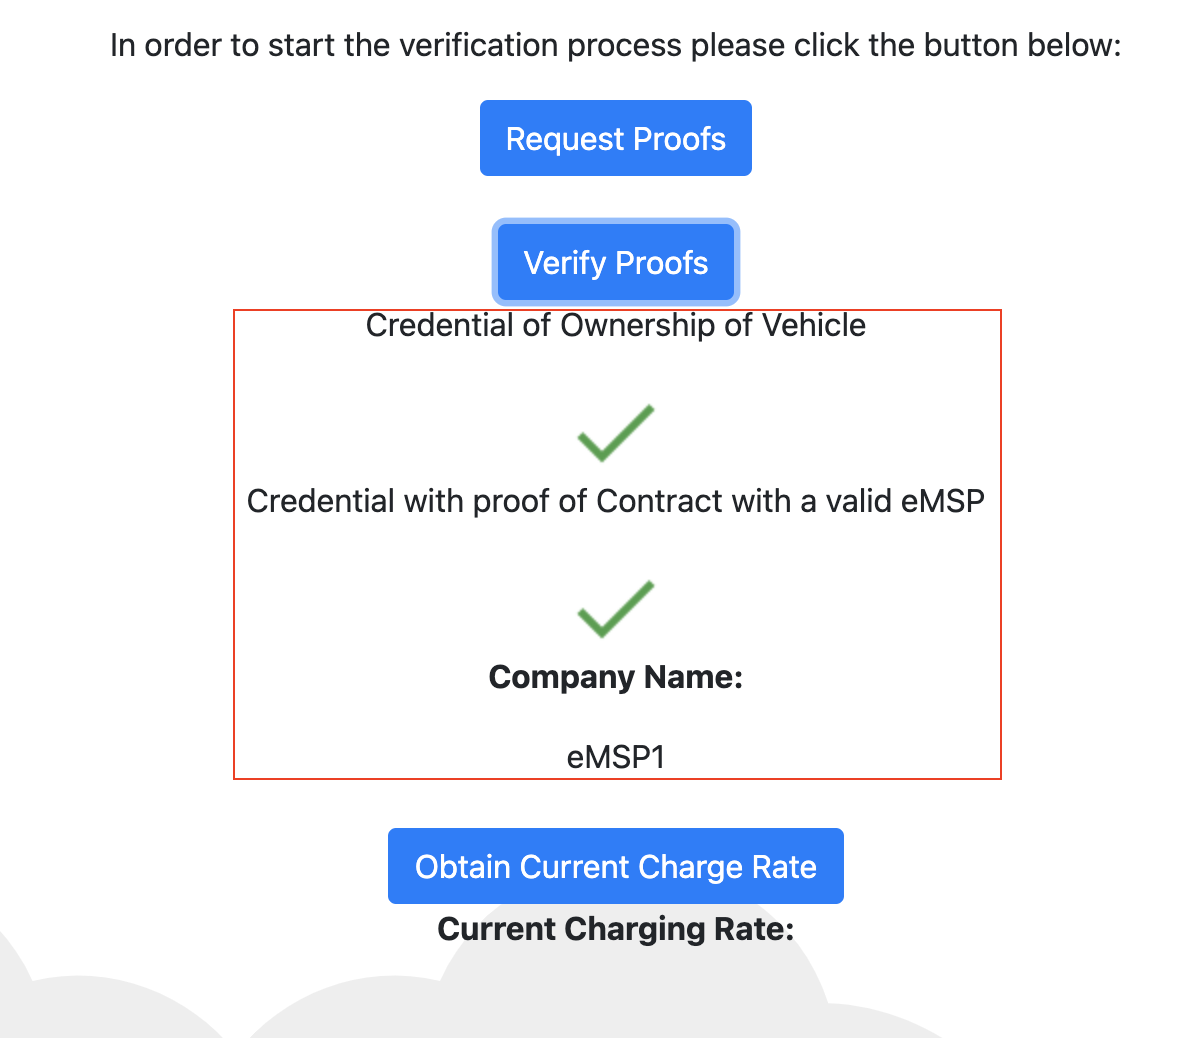
\includegraphics[width=.9\linewidth]{images/Frontend/Charging/5.png}
  \caption[]{Verify that both credentials are valid on the dashboard}
  \label{fig:charging_screenshot_5}
\end{minipage}
\end{figure}

\begin{figure}[H]
\centering
\begin{minipage}{.5\textwidth}
  \centering
  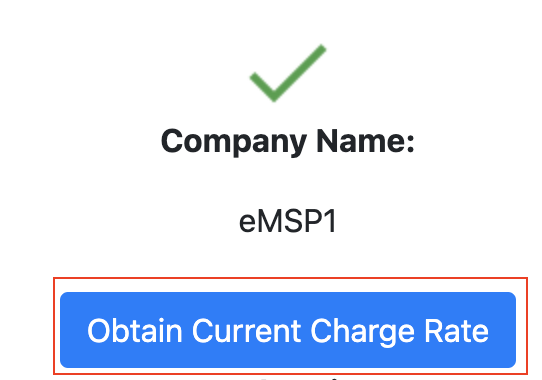
\includegraphics[width=.9\linewidth]{images/Frontend/Charging/6.png}
  \caption[]{Press the "Obtain Current Charge Rate" button}
  \label{fig:charging_screenshot_6}
\end{minipage}%
\begin{minipage}{.5\textwidth}
  \centering
  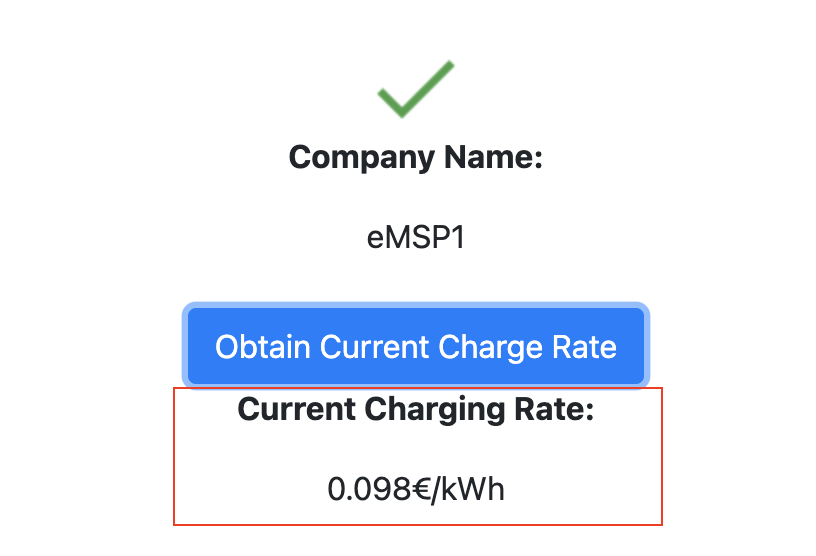
\includegraphics[width=.9\linewidth]{images/Frontend/Charging/7.png}
  \caption[]{Verify the kWh price on the dashboard}
  \label{fig:charging_screenshot_7}
\end{minipage}
\end{figure}

\begin{figure}[H]
\centering
\begin{minipage}{.5\textwidth}
  \centering
  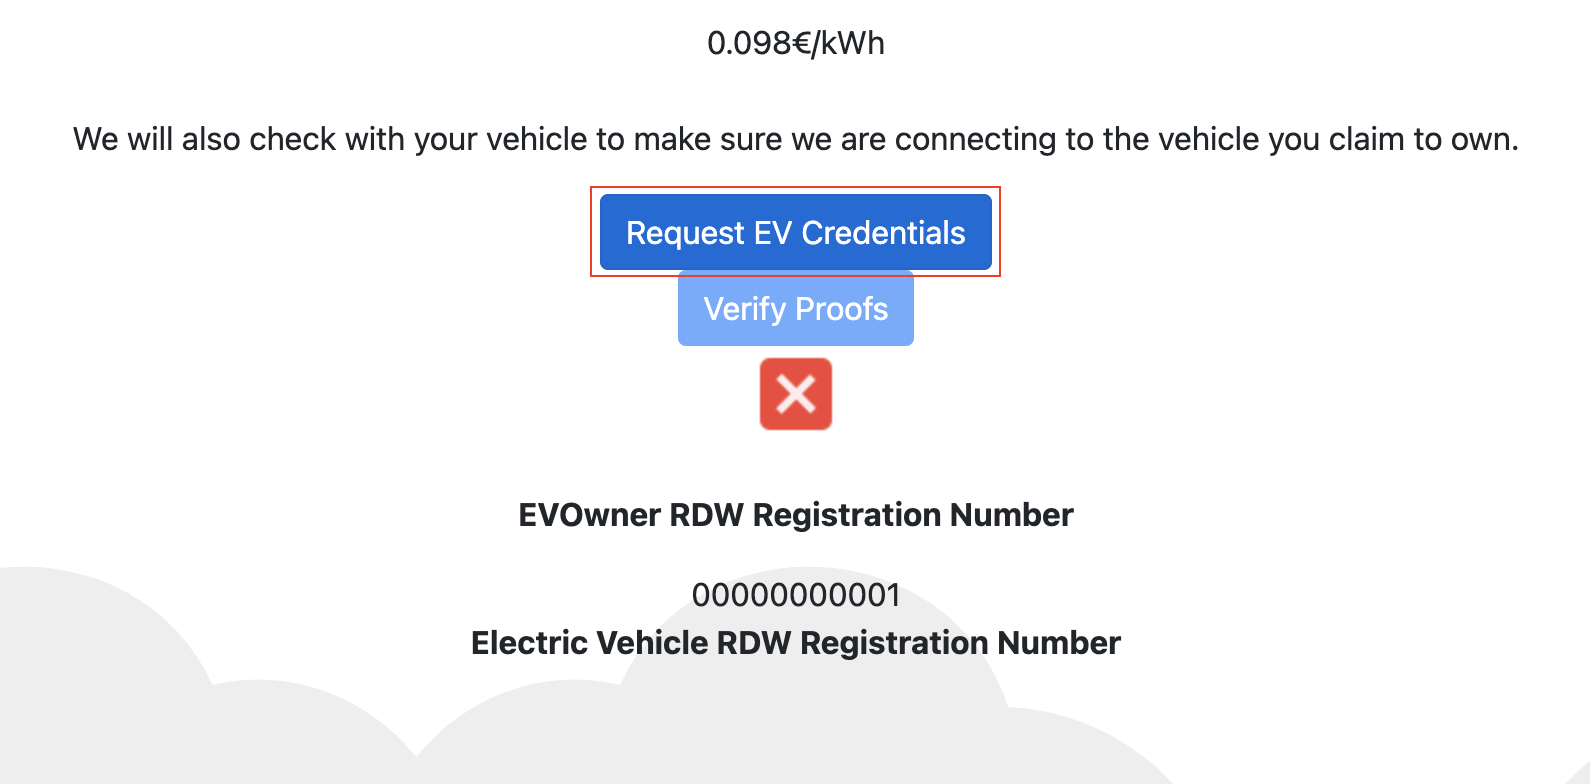
\includegraphics[width=.9\linewidth]{images/Frontend/Charging/8.png}
  \caption[]{Press the "Request EV Credentials" button}
  \label{fig:charging_screenshot_8}
\end{minipage}%
\begin{minipage}{.5\textwidth}
  \centering
  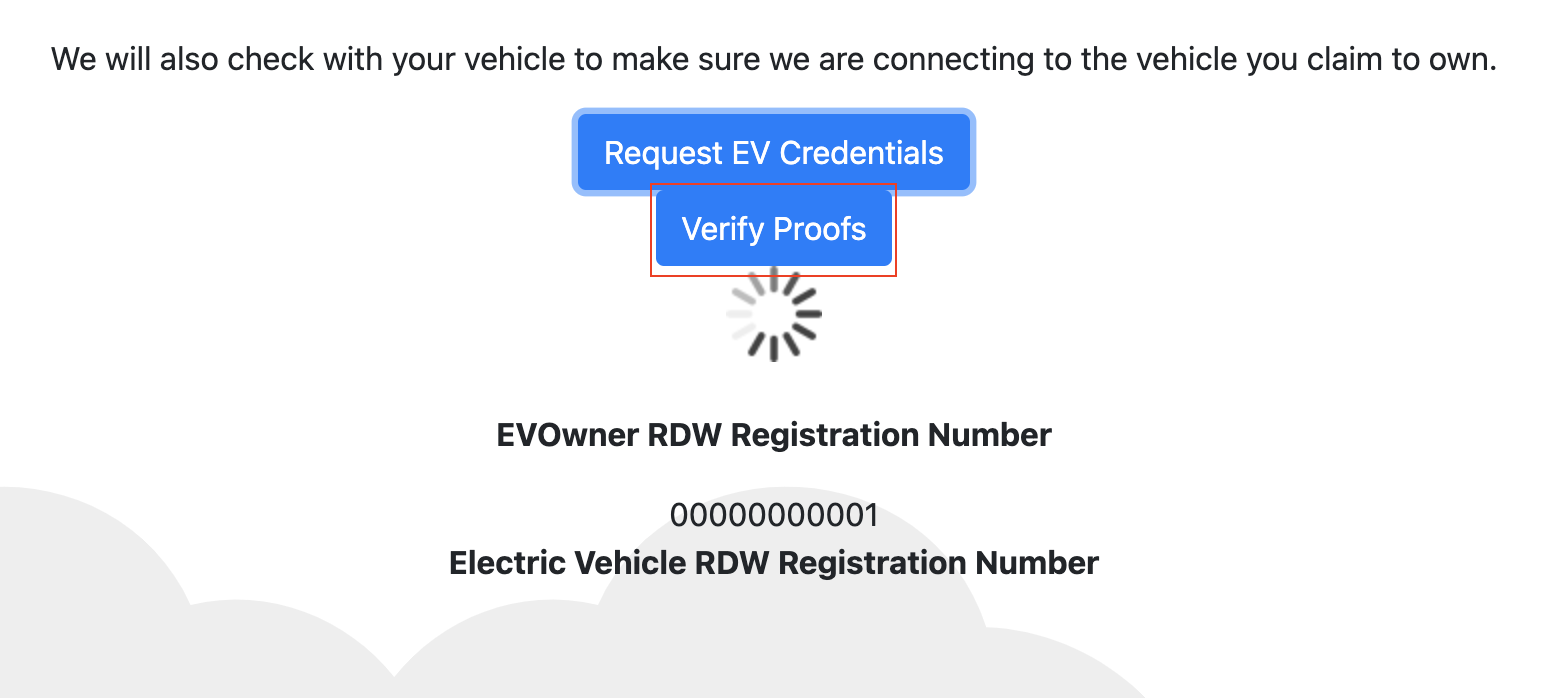
\includegraphics[width=.9\linewidth]{images/Frontend/Charging/9.png}
  \caption[]{Press the "Verify Proofs" button}
  \label{fig:charging_screenshot_9}
\end{minipage}
\end{figure}

\begin{figure}[H]
\centering
\begin{minipage}{.5\textwidth}
  \centering
  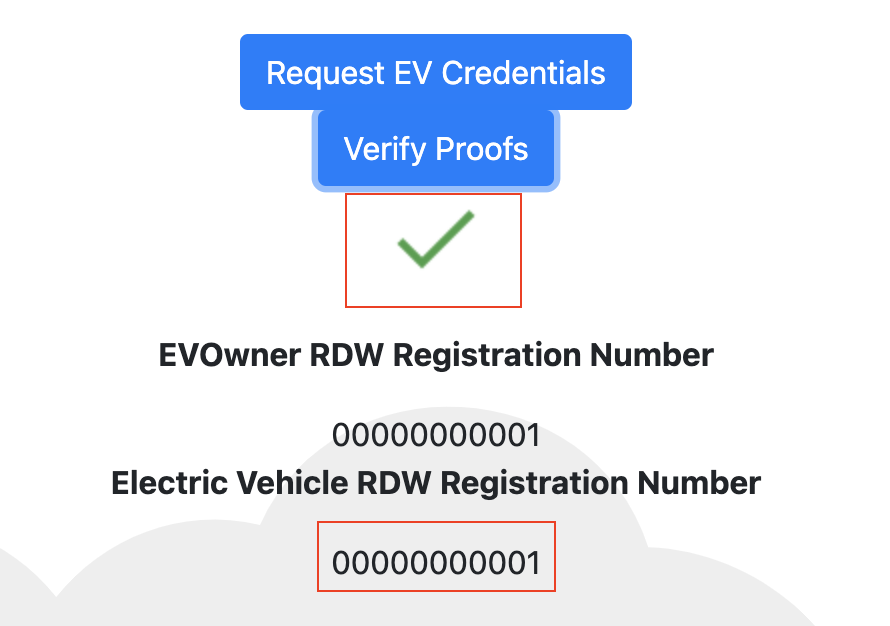
\includegraphics[width=.9\linewidth]{images/Frontend/Charging/10.png}
  \caption[]{Verify that the credential is valid on the dashboard and that the Registration Numbers match}
  \label{fig:charging_screenshot_10}
\end{minipage}%
\begin{minipage}{.5\textwidth}
  \centering
  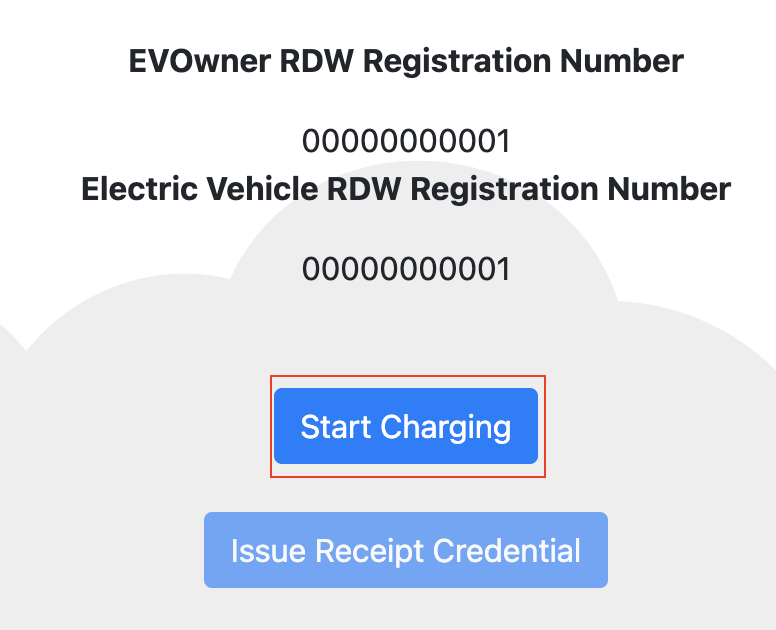
\includegraphics[width=.9\linewidth]{images/Frontend/Charging/11.png}
  \caption[]{Press the "Start Charging" button}
  \label{fig:charging_screenshot_11}
\end{minipage}
\end{figure}

\begin{figure}[H]
\centering
\begin{minipage}{.5\textwidth}
  \centering
  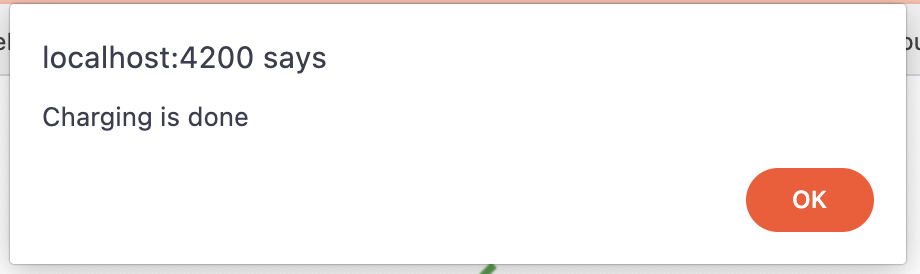
\includegraphics[width=.9\linewidth]{images/Frontend/Charging/12.png}
  \caption[]{Verify that charging has occurred on the dashboard}
  \label{fig:charging_screenshot_12}
\end{minipage}%
\begin{minipage}{.5\textwidth}
  \centering
  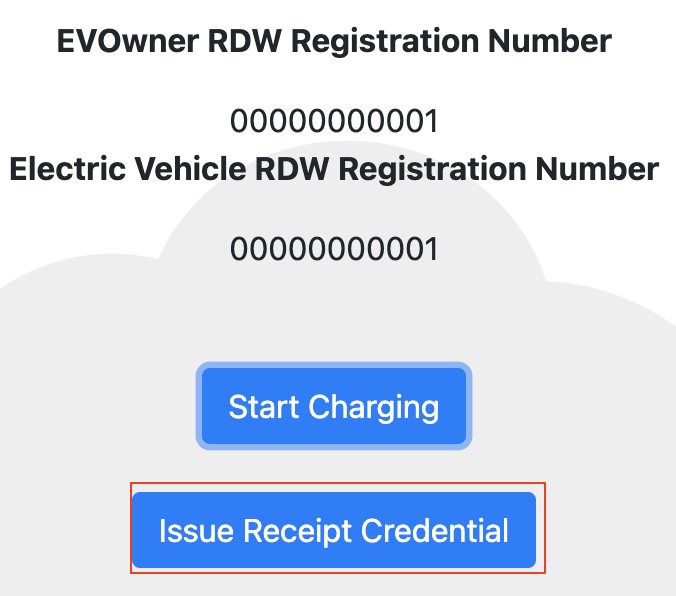
\includegraphics[width=.9\linewidth]{images/Frontend/Charging/13.png}
  \caption[]{Press the "Issue Receipt Credential" button}
  \label{fig:charging_screenshot_13}
\end{minipage}
\end{figure}

\begin{figure}[H]
\centering
\begin{minipage}{.33\textwidth}
  \centering
  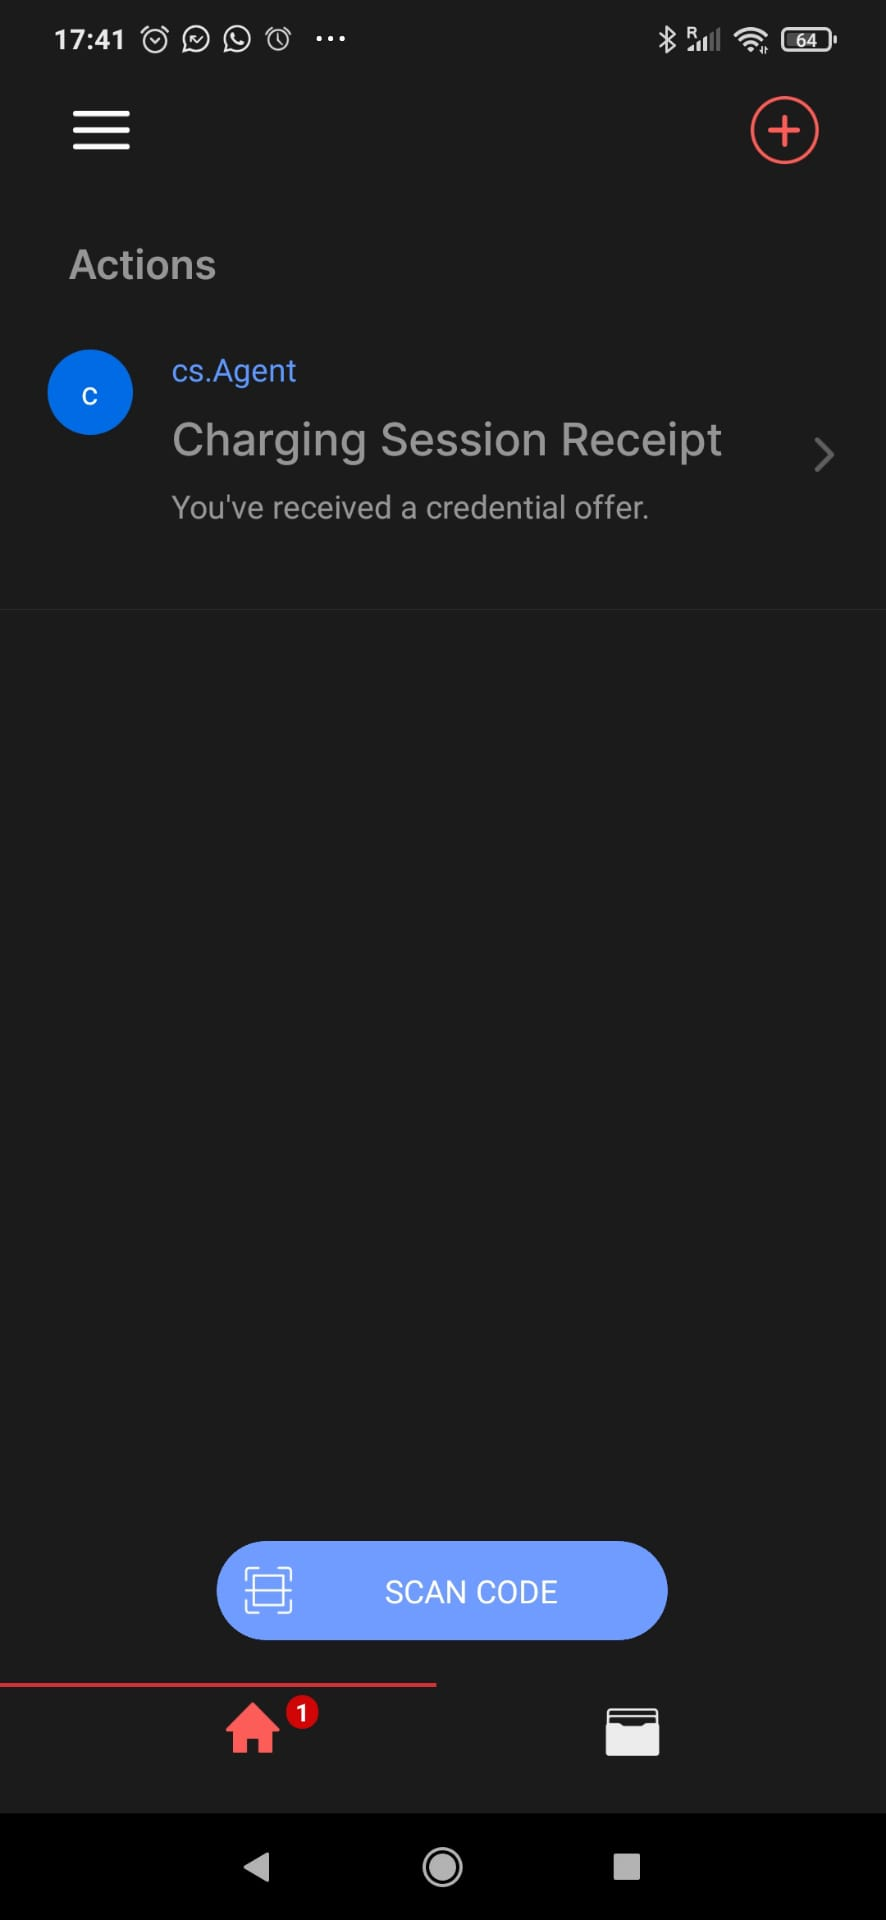
\includegraphics[width=.9\linewidth]{images/Frontend/Charging/14.0.jpeg}
  \caption[]{Receive the credential proposal on the Trinsic Wallet App}
  \label{fig:charging_screenshot_14.0}
\end{minipage}%
\begin{minipage}{.33\textwidth}
  \centering
  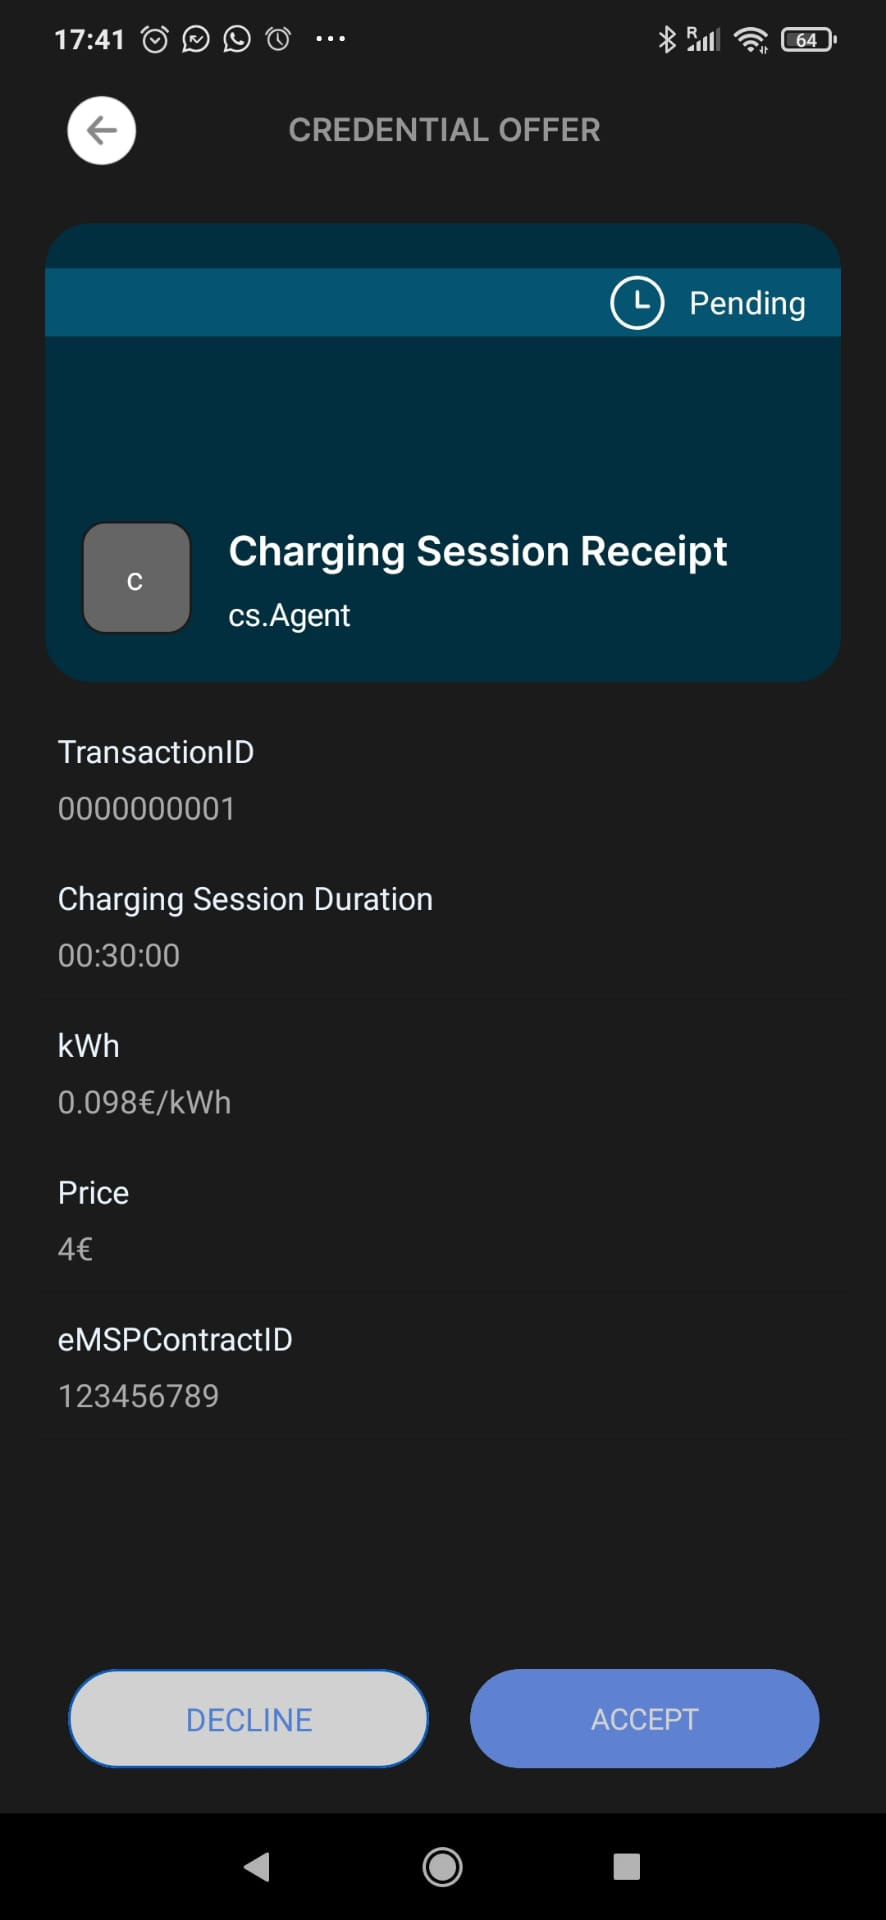
\includegraphics[width=.9\linewidth]{images/Frontend/Charging/14.1.jpeg}
  \caption[]{Accept the credential on the Trinsic Wallet App}
  \label{fig:charging_screenshot_14.1}
\end{minipage}
\end{figure}

\begin{figure}[H]
    \centering
    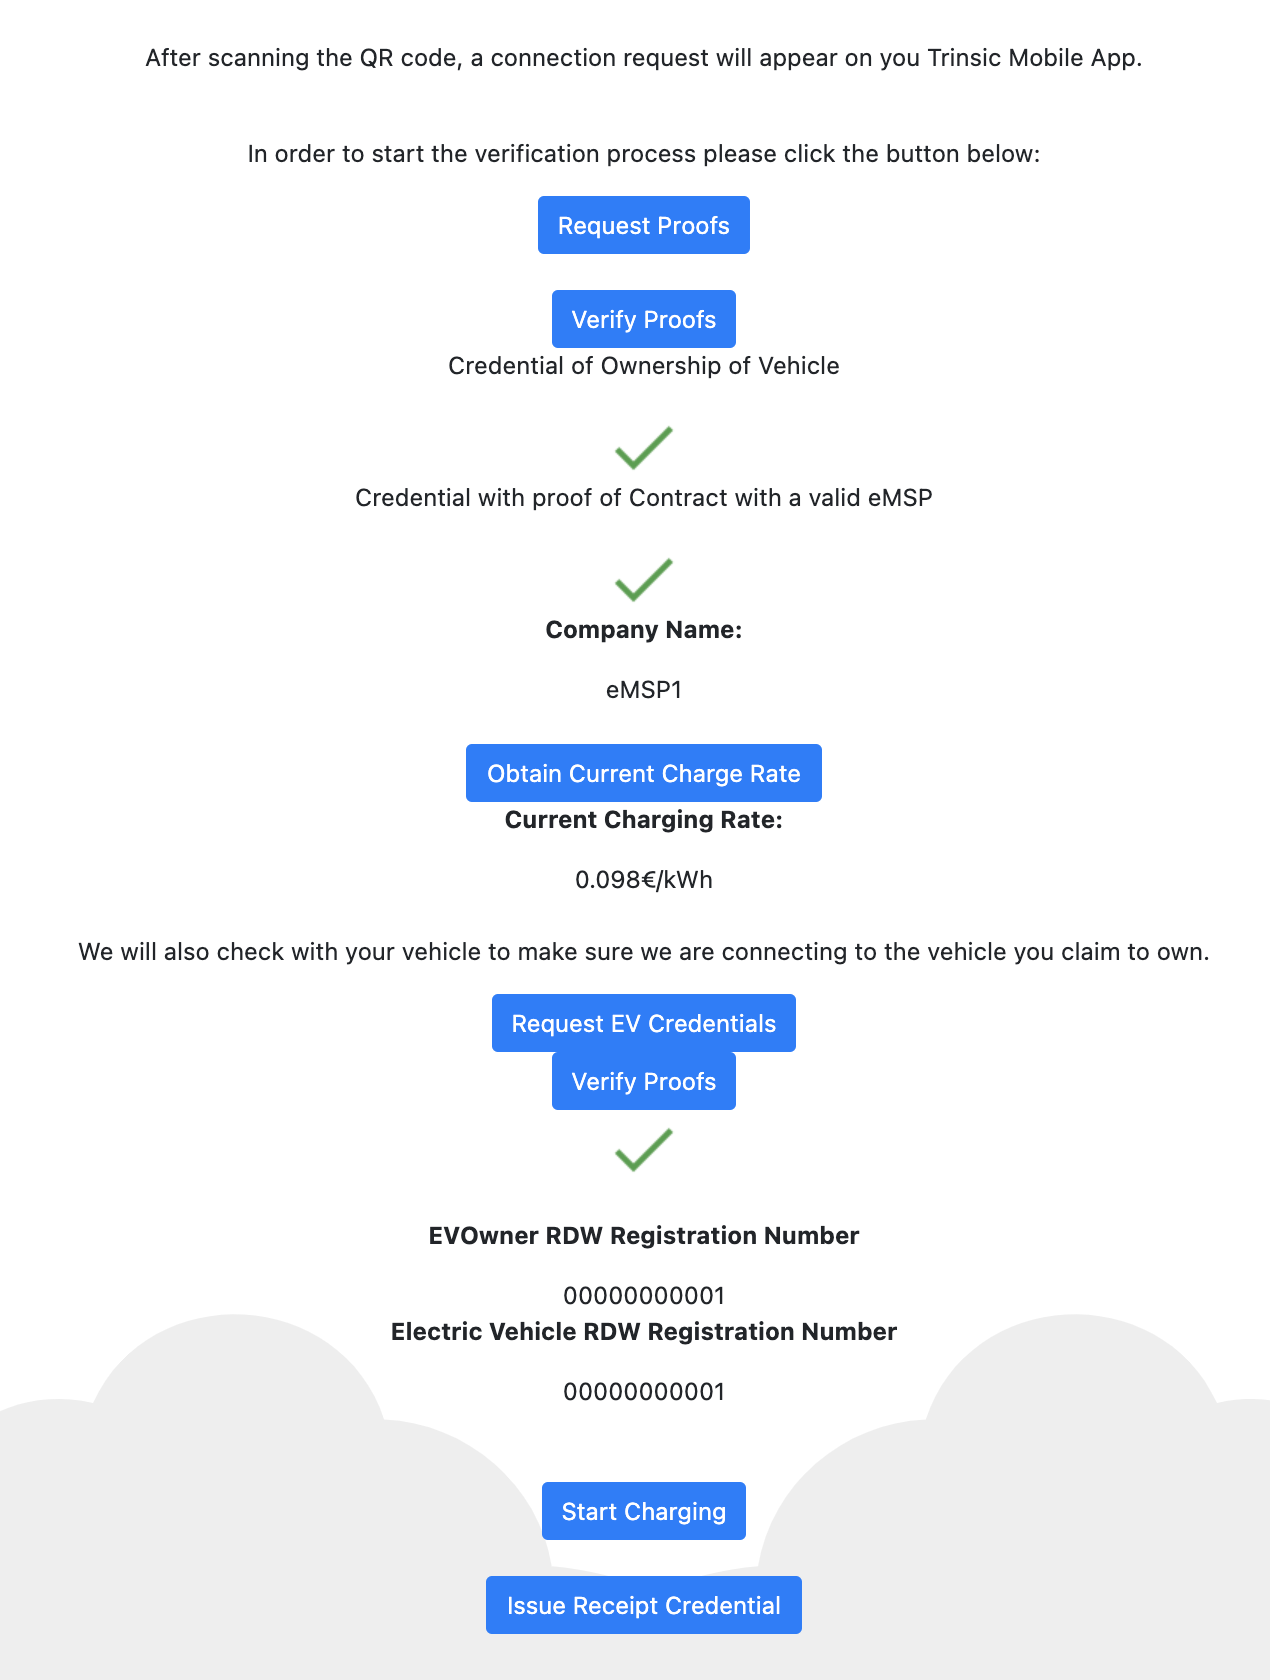
\includegraphics[width=0.6\linewidth]{images/Frontend/Charging/15.png}
    \caption[]{State of the dashboard at the end of a charging session}
    \label{fig:charging_screenshot_15}
\end{figure}

\newpage

\subsection{Aries Cloud Agent - Python Benchmark Runs}
\label{app:benchmark_runs}

In this appendix the commands used to obtain the average time of credentials are listed, followed by a small paragraph with additional information on connection times, revocation times, time to publish a schema and a credential definition.

\begin{itemize}
    \item \textit{./demo/run\_demo performance --count 1000 --mediation 2>\&1 | tee no\_revocation\_mediation\_1000.txt}
    \item \textit{./demo/run\_demo performance --count 1000 --revocation --tails-server-base-url http://host.docker.internal:6543 2>\&1 | tee revocation\_no\_mediation\_1000.txt }
    \item \textit{./demo/run\_demo performance --count 1000 2>\&1 | tee no\_revocation\_no\_mediation\_1000.txt}
    \item \textit{./demo/run\_demo performance --count 1000 --revocation --tails-server-base-url http://host.docker.internal:6543 --mediation 2>\&1 | tee revocation\_mediation\_1000.txt}
\end{itemize}

All the tests were made using the following laptop specifications:

\begin{itemize}
    \item Model Name:	MacBook Pro
    \item Model Identifier:	MacBookPro15,1
    \item Processor Name:	8-Core Intel Core i9
    \item Processor Speed:	2,3 GHz
    \item Number of Processors:	1
    \item Total Number of Cores:	8
    \item L2 Cache (per Core):	256 KB
    \item L3 Cache:	16 MB
    \item Hyper-Threading Technology:	Enabled
    \item Memory:	16 GB
    \item System Firmware Version:	1554.100.64.0.0 (iBridge: 18.16.14556.0.0,0)
    \item Docker Version: 20.10.5
\end{itemize}


\subsubsection{No Revocation + Mediation}

\begin{itemize}
    \item Startup duration: 15.14s
    \item Connect duration: 2.73s
    \item Publish duration: 14.46s
    \item Completed 1000 credential exchanges in 229.15s
    \item Average time per credential: 0.23s (4.36/s)
\end{itemize}

\subsubsection{Revocation + No Mediation}

\begin{itemize}
    \item Startup duration: 8.06s
    \item Connect duration: 0.21s
    \item Publish duration: 21.83s
    \item Completed 1000 credential exchanges in 232.92s
    \item Average time per credential: 0.23s (4.29/s)
\end{itemize}

\subsubsection{No Revocation + No Mediation}

\begin{itemize}
    \item Startup duration: 8.06s
    \item Connect duration: 0.19s
    \item Publish duration: 11.66s
    \item Completed 1000 credential exchanges in 229.45s
    \item Average time per credential: 0.23s (4.36/s)
\end{itemize}

\subsubsection{Revocation + Mediation}

\begin{itemize}
    \item Startup duration: 15.68s
    \item Connect duration: 2.72s
    \item Publish duration: 10.01s
    \item Completed 1000 credential exchanges in 263.33s
    \item Average time per credential: 0.26s (3.80/s)
\end{itemize}

\subsection{Requirement Evaluation}
\label{app:requirement_evaluation}

In this appendix, all of the requirements are discussed, presenting a table containing the requirements description, priority, status, arguments to support or contest the requirement and, when applicable, an alternative is briefly introduced to the presented arguments.

\begin{table}[H]
    \centering
    \begin{tabular}{lp{0.6\textwidth}}
         \textbf{\customlabel{evaluation:FR-1.1}{FR-1.1}} & Priority\\
         \hline\hline
         \textbf{Priority} & \textit{Must}\\
         \hline\hline
         \textbf{Status} & \greencheck\\
         \hline
         \textbf{Problem/issue} & The system must allow for an EV Owner to charge its EV at a CS\\
         \hline
         \textbf{Arguments} & The system still carries the capabilities for a client to charge its Electric Vehicle. \\
         \hline
         \textbf{Alternative(s)} & -\\
         \end{tabular}
         \caption{Evaluation of FR-1.1}
\end{table}

\begin{table}[H]
    \centering
    \begin{tabular}{lp{0.6\textwidth}}
         \textbf{\customlabel{evaluation:FR-1.2}{FR-1.2}} & Priority\\
         \hline\hline
         \textbf{Priority} & \textit{Should}\\
         \hline\hline
         \textbf{Status} &  \greencheck \\
         \hline
         \textbf{Problem/issue} & The rate at which the kWh is being sold to the EV Owner should be presented before the charging starts\\
         \hline
         \textbf{Arguments} & The current implementation of the system has the CS agent communicate to the CPO agent the company under which the client has a contract with, and receives a price rate back, displaying it to the user on the dashboard. \\
         \hline
         \textbf{Alternative(s)} & The price per kWh could be sent as a message to the user via the Trinsic Wallet App, instead of being presented on the screen.\\
         \end{tabular}
         \caption{Evaluation of FR-1.2}
\end{table}

\begin{table}[H]
    \centering
    \begin{tabular}{lp{0.6\textwidth}}
         \textbf{\customlabel{evaluation:FR-1.3}{FR-1.3}} & Priority\\
         \hline\hline
         \textbf{Priority} & \textit{Must}\\
         \hline\hline
         \textbf{Status} & \greencheck \\
         \hline
         \textbf{Problem/issue} & The EV Owner must be prompted to accept/reject the price of the kWh \\
         \hline
         \textbf{Arguments} & Although this is not actively implemented in the solution, given that the kWh price is presented to the user, it can refuse to charge the vehicle by walking out of the latter \\
         \hline
         \textbf{Alternative(s)} & In the future it would be interesting to have the user have an "accept" or "refuse" button, but that would not change the flow of the system\\
         \end{tabular}
         \caption{Evaluation of FR-1.3}
\end{table}

\begin{table}[H]
    \centering
    \begin{tabular}{lp{0.6\textwidth}}
         \textbf{\customlabel{evaluation:FR-1.4}{FR-1.4}} & Priority\\
         \hline\hline
         \textbf{Priority} & \textit{Could}\\
         \hline\hline
         \textbf{Status} & \greencheck \\
         \hline
         \textbf{Problem/issue} & At the end of a transaction, the EV Owner could receive proof of the transaction with the amount due\\
         \hline
         \textbf{Arguments} & In the new implementation of the system, the EV Owner receives a credential on his Trinsic Wallet App agent that contains information regarding the charging session.\\
         \hline
         \textbf{Alternative(s)} & -\\
         \end{tabular}
         \caption{Evaluation of FR-1.4}
\end{table}

\begin{table}[H]
    \centering
    \begin{tabular}{lp{0.6\textwidth}}
         \textbf{\customlabel{evaluation:FR-2.1}{FR-2.1}} & Priority\\
         \hline\hline
         \textbf{Priority} & \textit{Must}\\
         \hline\hline
         \textbf{Status} &  \greencheck \\
         \hline
         \textbf{Problem/issue} & A CS must belong to a CPO\\
         \hline
         \textbf{Arguments} & The Charging Station holds a credential that attests it is owned by the Charging Point Operator. \\
         \hline
         \textbf{Alternative(s)} & -\\
         \end{tabular}
         \caption{Evaluation of FR-2.1}
\end{table}

\begin{table}[H]
    \centering
    \begin{tabular}{lp{0.6\textwidth}}
         \textbf{\customlabel{evaluation:FR-2.2}{FR-2.2}} & Priority\\
         \hline\hline
         \textbf{Priority} & \textit{Must}\\
         \hline\hline
         \textbf{Status} &  \greencheck \\
         \hline
         \textbf{Problem/issue} & A CPO must have a contract with an eMSP\\
         \hline
         \textbf{Arguments} & The CPO agent holds a credential that attests a contract with an eMSP.\\
         \hline
         \textbf{Alternative(s)} & -\\
         \end{tabular}
         \caption{Evaluation of FR-2.2}
\end{table}

\begin{table}[H]
    \centering
    \begin{tabular}{lp{0.6\textwidth}}
         \textbf{\customlabel{evaluation:FR-2.3}{FR-2.3}} & Priority\\
         \hline\hline
         \textbf{Priority} & \textit{Must}\\
         \hline\hline
         \textbf{Status} &  \greencheck \\
         \hline
         \textbf{Problem/issue} & A CPO must have a contract with an EP to provide power to its Charging Stations\\
         \hline
         \textbf{Arguments} & The CPO agent holds a credential that attests a contract with an EP. \\
         \hline
         \textbf{Alternative(s)} & -\\
         \end{tabular}
         \caption{Evaluation of FR-2.3}
\end{table}

\begin{table}[H]
    \centering
    \begin{tabular}{lp{0.6\textwidth}}
         \textbf{\customlabel{evaluation:FR-3.1}{FR-3.1}} & Priority\\
         \hline\hline
         \textbf{Priority} & \textit{Should}\\
         \hline\hline
         \textbf{Status} &  \greencheck \\
         \hline
         \textbf{Problem/issue} & EV Owners should prove they are the owners of their EV to a CS\\
         \hline
         \textbf{Arguments} & In the current implementation of the system, the EV Owner and the EV both have a credential provided by the Transportation Agency that links both by a registrationID, as seen in Section~\ref{paragraph:ev_owner_and_ev_interactions_with_ssi}. \\
         \hline
         \textbf{Alternative(s)} & The fact that the link between the EV and the EV Owner is made with the use of a unique identifier might impose privacy-damaging practices, that need to be evaluated at a later stage.\\
         \end{tabular}
         \caption{Evaluation of FR-3.1}
\end{table}
\begin{table}[H]
    \centering
    \begin{tabular}{lp{0.6\textwidth}}
         \textbf{\customlabel{evaluation:FR-3.2}{FR-3.2}} & Priority\\
         \hline\hline
         \textbf{Priority} & \textit{Must}\\
         \hline\hline
         \textbf{Status} &  \greencheck\\
         \hline
         \textbf{Problem/issue} & EV Owners must attest they have a valid contract with an eMSP that the CS's CPO has a contract with\\
         \hline
         \textbf{Arguments} & The EV Owner is given a credential from the eMSP that attests the contract between the two, and is presented at a Charging Station for verification. \\
         \hline
         \textbf{Alternative(s)} & -\\
         \end{tabular}
         \caption{Evaluation of FR-3.2}
\end{table}

\begin{table}[H]
    \centering
    \begin{tabular}{lp{0.6\textwidth}}
         \textbf{\customlabel{evaluation:FR-3.3}{FR-3.3}} & Priority\\
         \hline\hline
         \textbf{Priority} & \textit{Could}\\
         \hline\hline
         \textbf{Status} &  \redcheckk\\
         \hline
         \textbf{Problem/issue} & An EV Owner could be made aware that the CS belongs to the CPO it claims\\
         \hline
         \textbf{Arguments} & Although the Charging Station holds a credential that attests it is owned by a specific CPO, that credential has not been included in the proof-of-concept, but could be added easily later on, with the support of a better mobile agent. \\
         \hline
         \textbf{Alternative(s)} & -\\
         \end{tabular}
         \caption{Evaluation of FR-3.3}
\end{table}
\begin{table}[H]
    \centering
    \begin{tabular}{lp{0.6\textwidth}}
         \textbf{\customlabel{evaluation:FR-3.4}{FR-3.4}} & Priority\\
         \hline\hline
         \textbf{Priority} & \textit{Should}\\
         \hline\hline
         \textbf{Status} &  \greencheck \\
         \hline
         \textbf{Problem/issue} & The process of setting up the connection and verifying credentials should be executed with the least EV Owner intervention as possible.\\
         \hline
         \textbf{Arguments} & The process of establishing a connection and verifying credentials has been reduced to a maximum of steps that abide to all of the requirements and does not incur in problem for the users, according to the data extracted from the experts evaluation in Section~\ref{subsec:qualitative_evaluatin_from_domain_experts}. \\
         \hline
         \textbf{Alternative(s)} & -\\
         \end{tabular}
         \caption{Evaluation of FR-3.4}
\end{table}

\begin{table}[H]
    \centering
    \begin{tabular}{lp{0.6\textwidth}}
         \textbf{\customlabel{evaluation:FR-4.1}{FR-4.1}} & Priority\\
         \hline\hline
         \textbf{Priority} & \textit{Must}\\
         \hline\hline
         \textbf{Status} &  \greencheck \\
         \hline
         \textbf{Problem/issue} & An EV and the information regarding its EV Owner must be registered with the TA in order for the EV to be on the roads and to be charged at a CS\\
         \hline
         \textbf{Arguments} & The EV and its EV Owner are registered at the Transportation Agency and are provided with credentials that attest these claims. \\
         \hline
         \textbf{Alternative(s)} & -\\
         \end{tabular}
         \caption{Evaluation of FR-4.1}
\end{table}

\begin{table}[H]
    \centering
    \begin{tabular}{lp{0.6\textwidth}}
         \textbf{\customlabel{evaluation:FR-5.1}{FR-5.1}} & Priority\\
         \hline\hline
         \textbf{Priority} & \textit{Must}\\
         \hline\hline
         \textbf{Status} &  \greencheck\\
         \hline
         \textbf{Problem/issue} & The system must not write PII in a publicly accessible data repository\\
         \hline
         \textbf{Arguments} & With the usage of the Hyperledger Indy and the Hyperledger Aries ecosystems, it is guaranteed that no Personally Identifiable Information is written on the blockchain, and that the data is only stored in wallets held by each entity as seen in Section~\ref{subsec:what_information_goes_onto_the_DLT?}. \\
         \hline
         \textbf{Alternative(s)} & -\\
         \end{tabular}
         \caption{Evaluation of FR-5.1}
\end{table}

\begin{table}[H]
    \centering
    \begin{tabular}{lp{0.6\textwidth}}
         \textbf{\customlabel{evaluation:FR-5.2}{FR-5.2}} & Priority\\
         \hline\hline
         \textbf{Priority} & \textit{Must}\\
         \hline\hline
         \textbf{Status} &  \greencheck \\
         \hline
         \textbf{Problem/issue} & Every credential issued must be verifiable using cryptographic proof\\
         \hline
         \textbf{Arguments} & With the cryptographic capabilities provided by Hyperledger Ursa to the solution, it is guaranteed that this solution employs state of the art cryptography practices, as seen in Section~\ref{subsubsec:hyperledger_indy_sovrin}.\\
         \hline
         \textbf{Alternative(s)} & -\\
         \end{tabular}
         \caption{Evaluation of FR-5.2}
\end{table}

\begin{table}[H]
    \centering
    \begin{tabular}{lp{0.6\textwidth}}
         \textbf{\customlabel{evaluation:FR-6.1}{FR-6.1}} & Priority\\
         \hline\hline
         \textbf{Priority} & \textit{Must}\\
         \hline\hline
         \textbf{Status} &  \redcheckk\\
         \hline
         \textbf{Problem/issue} & An EV Owner must be able to delegate (temporary) possession of its EV to another driver\\
         \hline
         \textbf{Arguments} & In the current implementation of the ACA-Py agents, there is a work in progress to implement delegated credentials, which will mitigate this requirement in a near future. \\
         \hline
         \textbf{Alternative(s)} & Issue a credential to each individual that will be the driver of the vehicle, which is impractical in real-life scenarios.\\
         \end{tabular}
         \caption{Evaluation of FR-6.1}
\end{table}


\begin{table}[H]
    \centering
    \begin{tabular}{lp{0.6\textwidth}}
         \textbf{\customlabel{evaluation:NFR-1.1}{NFR-1.1}} & Priority\\
         \hline\hline
         \textbf{Priority} & \textit{Must}\\
         \hline\hline
         \textbf{Status} & \textit{\textbf{-}}\\
         \hline
         \textbf{Problem/issue} & The system must scale according to the growth of the market. Supposing an adoption in the Dutch Market (300k EVs in 2020), the system must be able to support this number of vehicles and the estimated growth (3M EVs by 2030)\\
         \hline
         \textbf{Arguments} & This requirement can be validated with the results obtained in Section~\ref{subsec:benchmark_hyperledger_indy_and_aries} since the Sovrin network is able to withstand the current load without a loss of information. But for this requirement to be validated more tests need to be performed to the network to adjust the number of nodes needed to withstand such system scale. \\
         \hline
         \textbf{Alternative(s)} & -\\
         \end{tabular}
         \caption{Evaluation of NFR-1.1}
\end{table}

\begin{table}[H]
    \centering
    \begin{tabular}{lp{0.6\textwidth}}
         \textbf{\customlabel{evaluation:NFR-2.1}{NFR-2.1}} & Priority\\
         \hline\hline
         \textbf{Priority} & \textit{Should}\\
         \hline\hline
         \textbf{Status} &  \greencheck\\
         \hline
         \textbf{Problem/issue} & The system should be able to kickstart the charging process in a reasonable amount of time (no longer than the time required without VCs, less than 1 minute)\\
         \hline
         \textbf{Arguments} & The system has been timed in the charging station dashboard, and the process of charging could be started with less than 1 minute, depending on the user expertise with the technology. From the experts evaluation, the user experience has not been affected according to the results on Section~\ref{subsec:qualitative_evaluatin_from_domain_experts} \\
         \hline
         \textbf{Alternative(s)} & -\\
         \end{tabular}
         \caption{Evaluation of NFR-2.1}
\end{table}

\begin{table}[H]
    \centering
    \begin{tabular}{lp{0.6\textwidth}}
         \textbf{\customlabel{evaluation:NFR-2.2}{NFR-2.2}} & Priority\\
         \hline\hline
         \textbf{Priority} & \textit{Must}\\
         \hline\hline
         \textbf{Status} &  \greencheck\\
         \hline
         \textbf{Problem/issue} & The system must withstand multiple users accessing the system at the same time, with no loss of information.\\
         \hline
         \textbf{Arguments} & This requirement is assessed on a theoretical level, since no tests were made with concurrent agents performing the same flow. But, the capability of the system to handle concurrent users depends on the Hyperledger Indy network and not the agents, since each charging station will have one agent each, and therefore only have one session happening at the same time, which has been tested and proven to work. The network can withstand multiple agents writing at the same time as seen by the results on Section~\ref{subsec:benchmark_hyperledger_indy_and_aries}.  \\
         \hline
         \textbf{Alternative(s)} & -\\
         \end{tabular}
         \caption{Evaluation of NFR-2.2}
\end{table}

\begin{table}[H]
    \centering
    \begin{tabular}{lp{0.6\textwidth}}
         \textbf{\customlabel{evaluation:NFR-2.3}{NFR-2.3}} & Priority\\
         \hline\hline
         \textbf{Priority} & \textit{Must}\\
         \hline\hline
         \textbf{Status} &  \greencheck \\
         \hline
         \textbf{Problem/issue} & The user must be presented with information on how to engage with the CS in less than 5 seconds.\\
         \hline
         \textbf{Arguments} & As soon as the user arrives at the Charging Station, a call is made to the Charging Station agent to generate an invitation for the EV Owner to connect. This action occurs asynchronously and takes less than 2 seconds to appear.\\
         \hline
         \textbf{Alternative(s)} & -\\
         \end{tabular}
         \caption{Evaluation of NFR-2.3}
\end{table}

\begin{table}[H]
    \centering
    \begin{tabular}{lp{0.6\textwidth}}
         \textbf{\customlabel{evaluation:NFR-2.4}{NFR-2.4}} & Priority\\
         \hline\hline
         \textbf{Priority} & \textit{Should}\\
         \hline\hline
         \textbf{Status} &  \greencheck \\
         \hline
         \textbf{Problem/issue} & The process of validation the client’s credentials should not take longer than the original method (designed for 2 seconds, with the worst case scenario being 30 seconds)\\
         \hline
         \textbf{Arguments} & Following the work made on Section~\ref{subsec:benchmark_hyperledger_indy_and_aries} regarding the benchmarks of the ACA-Py agents and the results, this requirement can be marked as fulfilled. \\
         \hline
         \textbf{Alternative(s)} & -\\
         \end{tabular}
         \caption{Evaluation of NFR-2.4}
\end{table}

\begin{table}[H]
    \centering
    \begin{tabular}{lp{0.6\textwidth}}
         \textbf{\customlabel{evaluation:NFR-3.1}{NFR-3.1}} & Priority\\
         \hline\hline
         \textbf{Priority} & \textit{Should}\\
         \hline\hline
         \textbf{Status} &  \greencheck\\
         \hline
         \textbf{Problem/issue} & The system should be constantly updated to mitigate the risk of quantum-attacks, by employing state-of-the art cryptography\\
         \hline
         \textbf{Arguments} & The current implementation of the Hyperledger Indy and Aries frameworks are based on another project from the Hyperledger ecosystem, Ursa. This project is the cryptographic core of both projects and is constantly updated to provide state-of-the-art security to both solutions.  \\
         \hline
         \textbf{Alternative(s)} & -\\
         \end{tabular}
         \caption{Evaluation of NFR-3.1}
\end{table}

\begin{table}[H]
    \centering
    \begin{tabular}{lp{0.6\textwidth}}
         \textbf{\customlabel{evaluation:NFR-3.2}{NFR-3.2}} & Priority\\
         \hline\hline
         \textbf{Priority} & \textit{Must}\\
         \hline\hline
         \textbf{Status} & \textbf{-}\\
         \hline
         \textbf{Problem/issue} & The system must comply with Dutch regulations, including GDPR\\
         \hline
         \textbf{Arguments} & Although blockchain and the information that gets written to the DLT, as discussed in Section~\ref{subsec:what_information_goes_onto_the_DLT?}, do provide GDPR compliance, two matters on the solution do not. The two latter have been assessed in the Limitations chapter (Section~\ref{subsubsec:limitations}) and hence the requirement has been marked with \textbf{"-"}. \\
         \hline
         \textbf{Alternative(s)} & Discussed in the Limitations chapter.\\
         \end{tabular}
         \caption{Evaluation of NFR-3.2}
\end{table}

\begin{table}[H]
    \centering
    \begin{tabular}{lp{0.6\textwidth}}
         \textbf{\customlabel{evaluation:NFR-3.3}{NFR-3.3}} & Priority\\
         \hline\hline
         \textbf{Priority} & \textit{Must}\\
         \hline\hline
         \textbf{Status} &  \greencheck\\
         \hline
         \textbf{Problem/issue} & The system must be protected against forgery of identity, so that in the case of theft of identity the malicious party cannot use the system\\
         \hline
         \textbf{Arguments} & The core principals of SSI and the Verifiable Credentials allow to comply with this requirement, since each credential is cryptographically signed and there is no way to tamper this information or forge it, unless a wallet is taken hostage by a malicious party. But even in these circumstances, biometrics could be used as a Two-Factor Authentication method. \\
         \hline
         \textbf{Alternative(s)} & -\\
         \end{tabular}
         \caption{Evaluation of NFR-3.3}
\end{table}

\begin{table}[H]
    \centering
    \begin{tabular}{lp{0.6\textwidth}}
         \textbf{\customlabel{evaluation:NFR-4.1}{NFR-4.1}} & Priority\\
         \hline\hline
         \textbf{Priority} & \textit{Must}\\
         \hline\hline
         \textbf{Status} &  \greencheck\\
         \hline
         \textbf{Problem/issue} & A CS must have an active internet connection to authenticate the EV Owner\\
         \hline
         \textbf{Arguments} & Although not actively evaluated, in Section~\ref{subsubsec:evaluation_non_functional_requirements} a discussion is conducted to why this requirement can be fulfilled if applied in the Netherlands.\\
         \hline
         \textbf{Alternative(s)} & Perform more research to assess the current state of charging station connectivity in more regions where this solution might be applied. \\
         \end{tabular}
         \caption{Evaluation of NFR-4.1}
\end{table}

\begin{table}[H]
    \centering
    \begin{tabular}{lp{0.6\textwidth}}
         \textbf{\customlabel{evaluation:NFR-4.2}{NFR-4.2}} & Priority\\
         \hline\hline
         \textbf{Priority} & \textit{Must}\\
         \hline\hline
         \textbf{Status} &  \greencheck\\
         \hline
         \textbf{Problem/issue} & The systems implementation must allow for as many agent implementations as possible, opting for solutions that favor interoperability\\
         \hline
         \textbf{Arguments} & This requirement is fulfilled since the goal of Hyperledger Indy and Aries is to provide an interoperable ecosystem that is not vendor-locked. Any agent that complies with the current Verifiable Credentials standards is capable of interacting with the Hyperledger Indy network, and that is why this requirement is fulfilled. \\
         \hline
         \textbf{Alternative(s)} & -\\
         \end{tabular}
         \caption{Evaluation of NFR-4.2}
\end{table}

\begin{table}[H]
    \centering
    \begin{tabular}{lp{0.6\textwidth}}
         \textbf{\customlabel{evaluation:NFR-4.3}{NFR-4.3}} & Priority\\
         \hline\hline
         \textbf{Priority} & \textit{Must}\\
         \hline\hline
         \textbf{Status} &  \greencheck\\
         \hline
         \textbf{Problem/issue} & The system must offer a 97\% uptime guarantee\\
         \hline
         \textbf{Arguments} & Following the evaluation performed on the Hyperledger Indy network in Section~\ref{subsec:benchmark_hyperledger_indy_and_aries}, the current best example of an Indy network has more than 97\% uptime, which leads to believe that it is capable of handling this availability requirements.\\
         \hline
         \textbf{Alternative(s)} & -\\
         \end{tabular}
         \caption{Evaluation of NFR-4.3}
\end{table}


\newpage

